\RequirePackage[l2tabu, orthodox]{nag}
\documentclass[a4paper,12pt, openright, twoside]{report}
\usepackage{listings}
\usepackage{color} %red, green, blue, yellow, cyan, magenta, black, white
\usepackage[T1]{fontenc}
\usepackage[utf8]{inputenc}
\usepackage[american]{babel}
\usepackage[breaklinks=true,colorlinks=false,pdfborder={0 0 0}]{hyperref}
\usepackage{lmodern}
\usepackage{graphicx}
\usepackage{datetime2}
\usepackage{url}
%\usepackage{breakurl}
\usepackage{wrapfig}
\usepackage{subcaption}
\usepackage{microtype}
%\usepackage{inconsolata}
%\usepackage[lf]{MinionPro}
\usepackage{textcomp}
\usepackage{booktabs}
\usepackage{multirow}
\usepackage{amsmath}
\usepackage{amssymb}
\usepackage{cleveref}
\usepackage{courier}
\usepackage{xstring}
\usepackage{mathrsfs}
\usepackage{units}
\usepackage{threeparttable}
\usepackage[inline]{enumitem}
\usepackage{todonotes}
\usepackage{gensymb}
\usepackage{lipsum}
\usepackage{fancyhdr}
\usepackage[headsep=.5cm,headheight=1cm,left=3cm,right=2cm,top=3cm,bottom=2.5cm]{geometry}
\usepackage[numbib]{tocbibind}
\usepackage{appendix}
\usepackage{imakeidx}
\usepackage{tabularx}
\usepackage[ruled,vlined]{algorithm2e}
\usepackage[toc,acronym]{glossaries}
\usepackage{gensymb}
\usepackage{float}
% Set listing style
\lstdefinestyle{mystyle}{
captionpos=b,
frame=tb,
prebreak=\raisebox{0ex}[0ex][0ex]{\ensuremath{\hookleftarrow}},
aboveskip=20pt,
belowskip=20pt
}
\lstset{style=mystyle}

\definecolor{maroon}{rgb}{0.5,0,0}
\definecolor{darkgreen}{rgb}{0,0.5,0}
\lstdefinelanguage{XML}
{
  basicstyle=\ttfamily,
  morestring=[s]{"}{"},
  morecomment=[s]{?}{?},
  morecomment=[s]{!--}{--},
  commentstyle=\color{darkgreen},
  moredelim=[s][\color{black}]{>}{<},
  moredelim=[s][\color{red}]{\ }{=},
  stringstyle=\color{blue},
  identifierstyle=\color{maroon}
}

\makeindex
\indexsetup{level=\section,noclearpage}

\reversemarginpar
\setlength{\marginparwidth}{2cm}

\providecommand{\keywords}[1]{\textbf{\textit{Keywords: }} #1}
\def\UrlBreaks{\do\/\do-}
\definecolor{mygreen}{RGB}{28,172,0} % color values Red, Green, Blue
\definecolor{mylilas}{RGB}{170,55,241}


\lstset{language=Matlab,%
    basicstyle=\footnotesize\ttfamily,
    %basicstyle=\color{red},
    flexiblecolumns=true,
    breaklines=true,%
    morekeywords={matlab2tikz,tf,series,parallel,feedback},
    keywordstyle=\color{blue},%
    morekeywords=[2]{1}, keywordstyle=[2]{\color{black}},
    identifierstyle=\color{black},%
    stringstyle=\color{mylilas},
    commentstyle=\color{mygreen},%
    showstringspaces=false,%without this there will be a symbol in the places where there is a space
    numbers=left,%
    numberstyle={\tiny \color{black}},% size of the numbers
    numbersep=9pt, % this defines how far the numbers are from the text
    emph=[1]{for,end,break},emphstyle=[1]\color{red}, %some words to emphasise
    %emph=[2]{word1,word2}, emphstyle=[2]{style},    
}


\title{Agricultural Field Detection and Coverage Path Planning for an Unmanned Aerial Vehicle}
\author{Michael Rimondi}
\date{\today}


% Make the list of * output as SECTION rather than CHAPTER
\makeatletter
\newcommand\renewlistof[3]%
   {\renewcommand#1%
      {\section{#3}%
       %\addcontentsline{toc}{chapter}{#3}%
       \markboth{#3}{#3}%
       \@starttoc{#2}%
      }%
   }

\makeatother
\renewlistof\listoffigures{lof}{\listfigurename}
\renewlistof\listoftables{lot}{\listtablename}
\renewlistof\lstlistoflistings{lstlol}{\lstlistlistingname}

%!TEX root = bambi-thesis.tex

\def\maketitle{\begingroup % Create the command for including the title page in the document
% \centering % Center all text
% \thispagestyle{empty} 
% \vspace*{4cm}

% \rule{\textwidth}{1.6pt}\vspace*{-\baselineskip}\vspace*{2pt} % Thick horizontal line
% \rule{\textwidth}{0.4pt}\\[\baselineskip] % Thin horizontal line

% {\LARGE  \textsc{\@title}}\\[0.2\baselineskip] % Title

% \rule{\textwidth}{0.4pt}\vspace*{-\baselineskip}\vspace{3.2pt} % Thin horizontal line
% \rule{\textwidth}{1.6pt}\\[\baselineskip] % Thick horizontal line

% \scshape % Small caps
% \subtitle\\[1.5\baselineskip] % Tagline(s) or further description
% Bologna, \@date \par % Location and year

% \vspace*{2\baselineskip} % Whitespace between location/year and editors

% \subject

% \vspace*{2\baselineskip} % Whitespace between location/year and editors

% Edited by \\[\baselineskip]
% {\Large \@author\\[2\baselineskip]\par} % Editor list
% \includegraphics[width=.15\textwidth]{figures/universitiy-of-bologna-logo.jpg}\\[0.3\baselineskip]
% {\itshape Università di Bologna\par} % Editor affiliation
% \vfill % Whitespace between editor names and publisher logo



% \vspace*{\baselineskip} % Whitespace between location/year and editors

% \textit{\textbf{Supervisors:}\\[\baselineskip]\textsc{\mentors}}

\thispagestyle{empty} 
\begin{center}
{{\Large{\textsc{Alma Mater Studiorum $\cdot$ Università di
Bologna}}}}\\
\vskip - 5pt
\rule{\textwidth}{0.1mm}
\rule[0.5cm]{\textwidth}{0.6mm}
\vskip -13pt
{\small{\textsc{Scuola di Ingegneria e Architettura\\
\vspace{4mm}
\small{Dipartimento di Ingegneria dell'Energia Elettrica e dell'Informazione \\
"Guglielmo Marconi" – DEI\\}}}}
% 
% 
% SCUOLA DI INGEGNERIA E ARCHITETTURA
% DIPARTIMENTO DI
% INGEGNERIA DELL'ENERGIA ELETTRICA E DELL'INFORMAZIONE
% "Guglielmo Marconi"
% DEI
% 
\vspace{15mm}
{\large{\textsc{{Corso di Laurea in Ingegneria dell'Automazione}}}}
\vskip 5mm
\rule{10cm}{0.4mm}
\rule[0.5cm]{10cm}{0.1mm}\\
\vskip -5pt
{\LARGE\textbf{{Agricultural Field Detection}}}\\
\vspace{.5em}
{\LARGE{\textbf{{and Path Planning}}}}\\
\vspace{.5em}
{\LARGE{\textbf{{for an Unmanned Aerial Vehicle}}}}\\
%\vspace{3mm}
%{\LARGE{\textbf{ --}}}\\
\vskip -2pt
\rule{10cm}{0.1mm}
\rule[0.5cm]{10cm}{0.4mm}\\
\vspace{5mm} {\large{\textsc{Progetto di Laurea}}}
\end{center}
\vspace{8mm}
\centering

\includegraphics[width=.25\textwidth]{figures/university-of-bologna.pdf}
\vfill
\par
\noindent
\begin{minipage}[t]{0.47\textwidth}
{\large{\textit{Relatore:}}\\
{\textbf{Chiar.mo Prof. Lorenzo Marconi}}}\\
\vskip 8pt
{\large{\textit{Correlatore:}}\\
{\textbf{Prof. Nicola Mimmo}}}
\end{minipage}
\hfill
\begin{minipage}[t]{0.47\textwidth}\raggedleft
{\large{\textit{Presentato da:}}\\
%\vspace{2mm}
{\textbf{Michael Rimondi}}}
\end{minipage}
\vspace{22mm}
\begin{center}
{\large{\textsc{II Sessione\\%inserire il numero della sessione in cui ci si laurea
Anno Accademico 2017/2018}}}%inserire l'anno accademico a cui si è iscritti
\end{center}



\newpage

\endgroup}
\makeatother


% clear fancy hdr spaces
\fancyhf{}
\renewcommand*{\sectionmark}[1]{ \markright{\thesection\ ##1} }
% \fancyhead[LE,RO]{\rightmark}
\fancyhead[LO,RE]{\leftmark}
\fancyfoot[C]{\thepage}
\pagestyle{fancy}

%%%%%%%%%%%%%%%%%%%%%%%%%%Acronyms list BEGIN%%%%%%%%%%%%%%%%%%%%%%%%%%
\makeglossaries
\newacronym{uav}{UAV}{Unmanned Aerial Vehicle}
\newacronym{ros}{ROS}{Robot Operating System}
\newacronym{cpp}{CPP}{Coverage Path Planning}
\newacronym{wgs84}{WGS84}{World Geodetic System of 1984}
\newacronym{utm}{UTM}{Universal Transverse of Mercator}
\newacronym{sitl}{SITL}{Software-In-The-Loop}
\newacronym{qgc}{QGC}{QGroundControl}
\newacronym{mavlink}{MAVLink}{Micro Air Vehicle Link}
\newacronym{xml}{XML}{eXtensible Markup Language}
\newacronym{qml}{QML}{Qt Modeling Language}
\newacronym{kml}{KML}{Keyhole Markup Language}

%%%%%%%%%%%%%%%%%%%%%%%%%%%Acronyms list END%%%%%%%%%%%%%%%%%%%%%%%%%%%
\begin{document}

\setcounter{secnumdepth}{3}
\setcounter{tocdepth}{3}
\hypersetup{pageanchor=false}
\maketitle

%%%%%%%%%%%%%% REMOVE ME %%%%%%%%%%%%%%%%%
\thispagestyle{empty}
\listoftodos
\pagenumbering{roman}
\setcounter{page}{1}
\newpage
% %%%%%%%%%%%%%% REMOVE ME %%%%%%%%%%%%%%%%%

% \thispagestyle{empty}
% \setcounter{page}{2}
% \cleardoublepage


\pagenumbering{roman}
\begin{abstract}
\addcontentsline{toc}{chapter}{Abstract}{}{}
\thispagestyle{plain}
\setcounter{page}{3}
\lipsum[43]
\vskip 2em
\keywords{One, Two}
\end{abstract}

\thispagestyle{empty}
\setcounter{page}{4}
\cleardoublepage


\renewcommand{\abstractname}{Abstract (italiano)}
\begin{abstract}
\addcontentsline{toc}{chapter}{Abstract (italiano)}{}{}
\thispagestyle{plain}
\setcounter{page}{5}
\lipsum[44]
\vskip 2em
\keywords{Uno, Due}
\end{abstract}



\thispagestyle{empty}
\cleardoublepage

% use pagestyle plain for content to put page numbers in the footer
\hypersetup{pageanchor=true}
\pagestyle{plain}
\tableofcontents


% Print Acronym list
\printglossary[type=\acronymtype]
\cleardoublepage

% begin content and use roman numbers for chapter,
% without including them in the section numbering (no I.1)
\pagestyle{fancy}
\pagenumbering{arabic}
\renewcommand{\thechapter}{\Roman{chapter}}
\renewcommand*\thesection{\arabic{section}}


\chapter{Introduction} % (fold)
\label{cha:introduction}

%!TEX root = bambi-thesis.tex



In this introduction it is first briefly described the motivation, objective and scope of the project this thesis has been developed in. Once the background has been well set and explained,it will be describe the specific subject of the thesis.


\section{Motivation} % (fold)
\label{sec:motivation}
 Deers gives birth to their offspring during April and May \cite{MowlingMortality}, often choosing meadows as they consider it a safe spot. This period is unfortunately the same in which meadows are cut. The results is that every year a great number of young deers fall victim of combine harvesters cutting hay. Germany counts about 100000 death every harvest season \cite{MowlingMortality}.
 The BambiSaver project was born aiming to provide an autonomous, fast and user friendly device able to search and locate, living creatures in agricultural areas. It is, as a matter of fact, difficult to locate small animals hidden in vast grasslands especially if they freeze when they feel under threat. For this specific reason the proposal design is based on a UAV (Unmanned Aerial Vehicle) \cite{ICAO} and more precisely a quad-copter equipped with a thermal camera.
 An aerial vehicle is, in fact, able to efficiently cover large surfaces way faster then any other ground alternatives and guarantees the best viewpoint for the specific kind of wildlife research. Moreover it has been chosen a copter rather than a fixed wing model for its holonomic properties which turns out to be very useful in upland regions as well as for small and irregular fields. It is basically why in search and rescue operations helicopters are often adopted instead of planes.

\subsection{Importance for Wildlife and for Agricultural}
\index{Agriculture}
In early hunting literature from as far back as the mid-19th century, references can be found to significant losses of breeding partridges and pheasants from the use of sickle and scythe. Due to the fierce competition in the agricultural sector, developments in agricultural technology have brought about a tremendous acceleration in mowing techniques, with tendency still rising. Today, mowing speed can even exceed 15 km/h, while at the same time ever-wider mowers are used. Nesting birds, young hares and fawns are regular victims of such mowers and even full-grown wild animals cannot always escape. Ever since the 1950s, the importance of silage meadows has increasingly taken precedence over the traditional hay harvest.

\subsection{Affected Species} % (fold)
\label{sub:affected_species}
Grassland is used by countless species of wildlife as food, cover and reproduction habitat. Apart from leverets, fawns and various field birds, small mammals, amphibians and insects all fall victim to the practice of early and more frequent mowing. Formerly reliable survival strategies proven successful over thousands of years have a devastating effect in mowing situations. The instinct of the brooding partridge hen to sit tight on her nest, or of the hare or fawn to freeze motionless, now prove fatal. The optimized patterns of predator avoidance behavior which wild animals have evolved can no longer keep up with the developments in modern cultivation techniques.
% subsection affected_species (end)
5de0697a03
\subsection{Measure to Reduce Wildlife Losses} % (fold)
\label{sub:measure_to_reduce_wildlife_losses}
 The most important factor influencing wildlife mortality is without doubt the time of mowing. On the other hand, economic considerations make this a crucial factor for the farmer, too. A late mowing is good for wildlife but not ideal for the farmer from the point of view of yield and quality. Yet there are some other factors in the mowing of arable land which offer potential for reducing wildlife losses \cite{MowlingMortality}:
\begin{itemize}
	\item \textit{Cutting height}: the higher the cut, the lower will be the losses suffered by crouching animals and nesting birds.
	\item \textit{Mowing direction}: mowing the field from the center outwards gives fully-grown wild animals the opportunity to escape.
	\item \textit{Mowing date}: late cuts,from mid-July onwards, reduce the losses to wildlife during the nesting and rearing period.
	\item \textit{Mowing strategy}: mowing of partial areas, leaving edge strips unmown.
	\item \textit{Mowing frequency}: a longer interval between first and second cuttings reduces the mortality rate, especially for ground-nesting birds.
	\item \textit{Mowing technology}: cutter-bar mowers cause less harm to wild animals than rotary mowers.
\end{itemize}
 Another practical approach is the one adopted in a German wildlife rescue project which consists in deploying small aerial drones to find young deer hiding in tall grass.
% subsection measure_to_reduce_wildlife_losses (end)

\section{State of the art} % (fold)
\label{sec:state_of_the_art}
 During last years, the increasing interest and development of UAS (Unmanned Aircraft System) makes them affordable and suitable for many different applications. Specifically, in wildlife research, drones are frequently use as they are less expensive, quieter, and safer than traditional manned aircraft. Most studies we reviewed recorded minimal or no visible behavioral responses to UAS; however, UAS are capable of causing behavioral and physiological responses in wildlife when observing at close range. \cite{doi:10.1002/fee.1281}.\\
 For the case under-study, the "Flying Wildlife Finder", represents the state-of-the-art.
 The project, developed by the German Aerospace Center (DLR), is an application system which prevents accidents by detecting animals hidden in tall grass during the hay harvest. 
 The "Flying Wildlife Finder", a remotely controlled aerial drone equipped with sensors and a GPS link, is sent on a reconnaissance flight before mowing starts. A high resolution thermal imaging camera detects the temperature of animals hidden in the grass, which is higher than the ambient temperature of the field. Once the animal is located a search party is led to the fawn’s resting place with the help of GPS.
 This solution proves to be good as it is less time-consuming then using trained dog, while maintaining even higher "hit-rate", but it has the main drawback of requiring at least two specialists: one pilot and one camera operator that must be focused on the thermal video stream during the whole mission duration.

 
% section state_of_the_art (end)
 
 \section{Proposal Solution} % (fold)
 \label{sec:proposal_solution}
 In the following section it is briefly explained the goals and design guidelines of the project.
 % section proposal_solution (end)

 \subsection{Project Goals} % (fold)
 \label{sec:bambisaver_goals}
 The scope of BambiSaver is to design an integrated system capable to autonomously handle every steps of the mission so that it can be operated also by untrained personals. This must be guaranteed even in adverse environments, especially in uneven fields as it is in upland regions. \todo{????the idea was developed having the mountain of Trentino Altoadige in mind????}
 Along with this, it is of particular interest to keep modularity in every hardware and software components. This is to permit easier implementation of new features or improvements.
 All this guidelines \todo{sinonimo per dire idee alla bass} have been taken into account during the design and implementation stages (i.e. ROS as framework for the on-board computer).

 \subsubsection{Software Design concept} % (fold)
 \label{ssub:software_design}
 The raspberry Pi 3 it is used as on-board computer, it runs ROS and manages the transition between the different mission's phases. The software develops according to the usual ROS philosophy \cite{288}, thus it is composed of five nodes implementing every mission component as an independent module. \autoref{fig:rqtgraph} displays all the nodes and the related topics used to let them communicate.
\begin{figure}[ht]
    \centering
    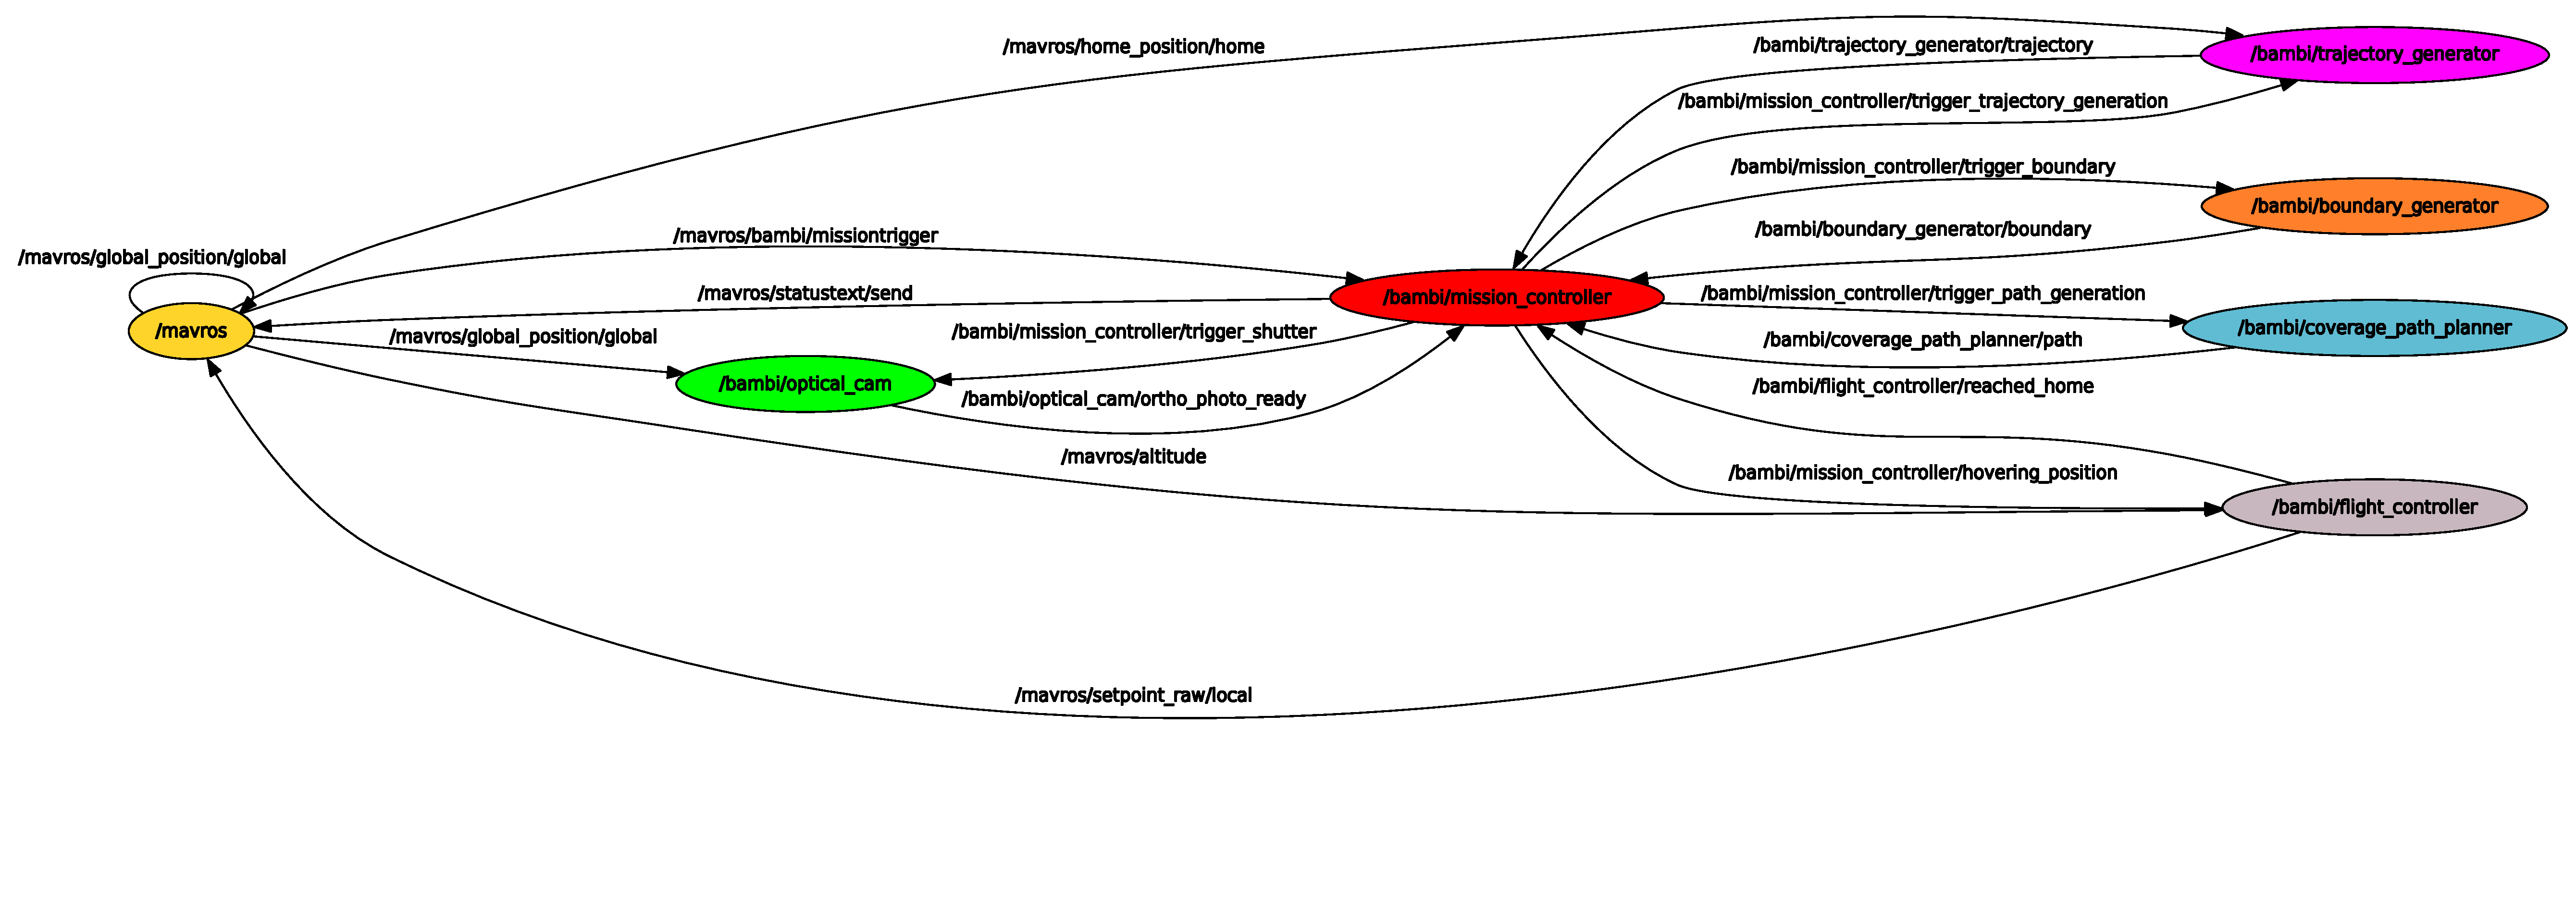
\includegraphics[width=1.4\textwidth, angle=270]{figures/C1/rqtgraph.eps}
    \caption{Nodes and Topics graph}
    \label{fig:rqtgraph}
\end{figure}\\
 In the following chapter the thesis will focus, exclusively on two problems:
 \begin{itemize}
  	\item \textit{Geo-referencing the mission's environment and get the field boundary}. This is of great importance, as it define the mission's range which is fundamental for every successive tasks.
  	\item \textit{Planning the coverage path}.It regards planning the geometric path so that the whole field of interest is covered by the sensor footprint.
  \end{itemize}
 
  % subsubsection software_design (end)

 

{}

 % Da mettere nel corpo della tesi NON INTRO
 % section bambisaver_goals (end)
% \section{Hardware Setup} % (fold)
% \label{sec:hardware_setup}
% The quadcopter (UAV) is equipped with:
% \begin{itemize}
% 	\item Pixhawk flashed with PX4 flight stack (see appendix \ref{appendix:pixhawk_flight_controller})
% 	\item NEO-M8n (GPS){}
% 	\item 3DR telemetry radio 433Hz (serial link between the UAV and the ground station)
% 	\item LidarLite V3 (altitude distance sensor) \cite{grm:lidarlite}
% 	\item Raspberry Pi 3b (Onboard computer running ROS over Ubuntu OS)
% \end{itemize} 
%  The ground station is composed by a common laptop running QGroundControl \todo{appendix or small description and features of QGC} application. The communication with the UAV uses the MAVLink protocol \cite{Mavlink} through an USB 433Hz telemetry radio .
% % section hardware_setup (end)

% \section{Software} % (fold)
% \label{sec:software}

% \todo{ROS, PX4 why we choose them}
% \todo{ROS design graph and explanation of each node}
% \todo{go deeply in ortho photo a}
% % section software (end)
% section  (end)
\section{Innovation} % (fold)
\label{sec:innovation}
 
 The approach 
The proposal device is an UAV \cite{ICAO}


\begin{align}
  \vec F &= \vec a \times \vec b\\
  {dof}_{rot} &= \sum_{i=1}^n (i-1) = n\, \frac{n-1}{2}
\end{align}


% section innovation (end)

% chapter introduction (end)



\chapter{Georeferencing the mission's environment} % (fold)
\label{cha:georeferencing_the_mission_s_environment}
%!TEX root = bambi-thesis.tex
In this chapter it is explained in details how the device obtain the information of the field boundary in form of a list of geographic coordinates. 
This important task will define the mission range of action which is used as input to the Coverage Path Planning module. It is thus important that the gathered information are rather precise and consistent or it will greatly impact the successive steps of the mission.\\
The process could be divided in two tasks:
\begin{itemize}
	\item Obtain a georeferenced photo displaying the entire meadow.
	\item Detect, trace and store the contour of the field from the georeferenced photo.
\end{itemize}

\section{Georeferencing a Photo} % (fold)
\label{sec:georeferenced_photo}
Before an aerial image can be used to support a site-specific application it is essential to perform the geometric corrections and geocoding. This is commonly called \textit{georeferencing} which enables the assignment of ground coordinates to the different features in the datasets. If the map projection \footnote{A map projection is a way to represent the curved surface
of the Earth on the flat surface of a map \cite{PosAccuracyGE}} (and map projection parameters) of the ground coordinates are known, equivalent geographic coordinates can be produced which enables positioning the features of the coverage into a World context. \cite{georefPractice}.
For this specific use case the final result is an orthophoto.

\subsection{Theory Background} % (fold)
\label{sub:theory_background}
\textit{"An orthophoto or orthoimage is an aerial photograph or image geometrically corrected ("orthorectified") such that the scale is uniform: the photo has the same lack of distortion as a map.}"\cite{orthophoto&GIS}\\

Unlike an uncorrected aerial photograph, an orthoimage can be used to measure true distances, because it is an accurate representation of the Earth's surface, having been adjusted for topographic relief, lens distortion, and camera tilt.
After the photo has been orthorectified it is georeferenced by transforming the local reference frame of the photo to the desired geographic coordinate system.\par
Among all the existing coordinate system the common \acrshort{wgs84} has been chosen as it is the standard in use by \acrshort{gps} (\acrlong{gps}). It consists of a three-dimensional Cartesian coordinate system and an associated ellipsoid, therefore \acrshort{wgs84} positions can be described as either XYZ Cartesian coordinates or latitude, longitude and ellipsoid height coordinates. The origin is the Geocentre (the centre of mass of the Earth), it is designed for positioning anywhere on Earth and as any other geographic coordinate system uses decimal degree as unit of measurement.\par
\todo{better explain WGS84 ref system???}
Spatial datasets, like any type of data, are prone to errors. Thus, three fundamental concepts have to be kept in mind: precision, bias and accuracy. Precision refers to the dispersion of positional random errors and it is usually expressed by a standard deviation. Bias, on the other hand, is associated with systematic errors and is usually measured by an average error that ideally should equal zero. Accuracy depends on both precision and bias and defines how close features on the map are from their true positions on the ground \cite{geoInformationSystem}. So, despite being frequently confused concepts, high precision does not necessarily mean high accuracy. But both depend greatly on the map scale. All maps have inherent positional errors, which depend on the methods used in the construction of the map. The scale is the ratio between a distance on the map and the corresponding distance on the ground. The maximum acceptable positional error (established by cartographic standards) is determined by the map scale.

\subsection{Ortho-rectification} % (fold)
\label{sub:ortho_rectification}
The goal of the ortho-rectification is to resample the pixels of an aerial photo to a coordinate system that is interpreted in a selected horizontal surface.
In georeferencing an aerial photo two distinct distortion effect should be corrected:
\begin{itemize}
	\item The perspective distortion, which is the result of the geometry of the photograph taking.
	\item The distortion effect of the relief and/or the surface.
\end{itemize}

The first one is addressed through camera calibration, which involves finding the focal length of the camera, principal point coordinates and lens distortion of each photo.
The second distortion effect can be corrected exploiting digital elevation model (DEM\footnote{The DEM is a raster of terrain elevations}) as shown in \autoref{fig:orthorectification}.
\begin{figure}[ht]
    \centering
    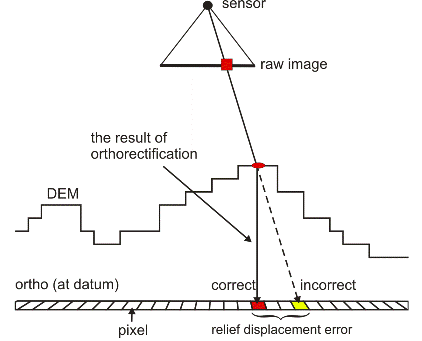
\includegraphics[width=0.6\textwidth]{figures/C2/Ortophoto.png}
    \caption{Orthorectification}
    \label{fig:orthorectification}
\end{figure}
The overall quality of the orthorectified image is therefore directly related to how accurate is the camera model and to the fidelity of the DEM. For this practical case the accuracy requirements of the georeferenced image is not so tight and so it has been decided, at first place, to use the ready-to-use Google Earth imagery database. Anyway in designing the mission work-flow it was predisposed the possibility to take an aerial photo of the entire site to georeference it.
% subsection ortho_rectification (end)

\subsection{Google Earth} % (fold)
\label{ssec:orthophoto_database}

\textit{"Google Earth is a virtual globe, map and geographical information program that was originally called Earth Viewer 3D, and was created by Keyhole, Inc, a Central Intelligence Agency (CIA) funded company acquired by Google in 2004. It maps the Earth by the superimposition of images obtained from satellite imagery, aerial photography and GIS 3D globe. Google Earth uses digital elevation model (DEM) data collected by NASA's Shuttle Radar Topography Mission (SRTM). The internal coordinate system of Google Earth is geographic coordinates (latitude/longitude) on the \acrfull{wgs84} datum i.e., the same datum that used by GPS."} \cite{PosAccuracyGE}.\\

Google Earth shows the earth surface as it looks from an elevated platform such as an airplane or orbiting satellite. The projection used to achieve this effect is called the General Perspective. This is similar to the Orthographic projection. Most of the high resolution imagery in Google Earth Maps is the Digital Globe Quickbird which is roughly 65cm pan sharpened. Google is actively replacing this base imagery with 2.5 m SPOT Image imagery and several higher resolution datasets.

The application is multi-platform and has an user friendly interface which among other provides tools to trace geographic feature such as shape, polygons and path. This turns out to be an essential feature in representing the field border which is after all, the final aim of this module. \todo{sinonimo di module???}.\\
The position accuracy of Google Earth was analyzed by Ahmed Ghazi whose selected 16 points in Khartoum
town. As of October 2012 The root mean square of the error results to be about $1.80m$ for horizontal position and $1.773m$ for height estimation.\cite{PosAccuracyGE} These results, while referring to only a specific region of the earth, are representative of the goodness of the data, especially considering they are available for free.\\
% subsection google_earth (end)
% section georeferenced_photo (end)

\section{Border Representation and Detection} % (fold)
\label{sec:border_detection_and_representation}
In order to obtain a digital representation of the border it is, first of all, important to define how to store the data in a file. Google Earth file format is the Keyhole Markup Language (KML).

\subsection{KML: Google Earth file format} % (fold)
\label{sub:kml_google_earth_file_format}
KML is an XML language focused on geographic visualization, including annotation of maps and images.
It became an international standard maintained by the Open Geospatial Consortium, Inc. (OGC).
KML can be used to:
\begin{itemize}
\item Annotate the Earth
\item Specify icons and labels to identify locations on the surface of the planet
\item Create different camera positions to define unique views for KML features
\item Define image overlays to attach to the ground or screen
\item Define styles to specify KML feature appearance
\item Write HTML descriptions of KML features, including hyperlinks and embedded images
\item Organize KML features into hierarchies
\item Locate and update retrieved KML documents from local or remote networklocations
\item Define the location and orientation of textured 3D objects
\end{itemize}

From a technical point of view, KML uses a tag-based structure based on XML standard \cite{bray06xml11}. All tags are case-sensitive and must be taken from the "KML Reference"\footnote{available at \url{https://developers.google.com/kml/documentation/kmlreference}}. \autoref{fig:KML-diagram} shows the most important attribute of a KML object. There are many object types, but for the application under interest some basic types like placemarks/points and lines are enough.
\begin{figure}[ht]
    \centering
    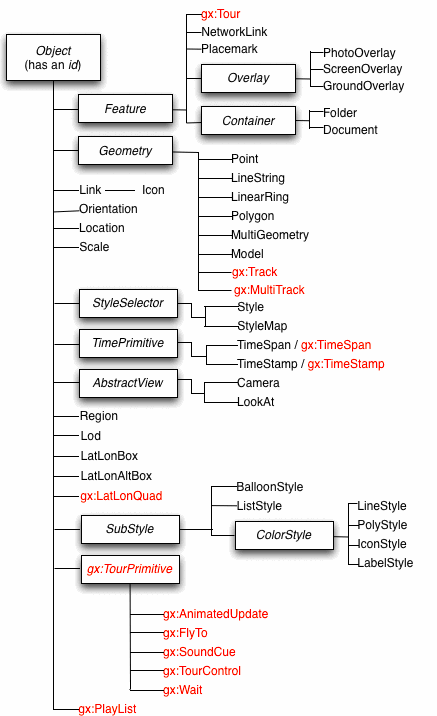
\includegraphics[width=0.5\textwidth]{figures/C2/KML-classTree.png}
    \caption{KML Object Hierarchy Diagram}
    \label{fig:KML-diagram}
\end{figure}

% subsection kml_google_earth_file_format (end)

\subsection{Field Border in KML} % (fold)
\label{sub:field_border_in_kml}
A border it is basically a close path having an undefined shape and therefore it cannot be represented using one polygon or other predefined geometric shapes. In KML such kind of geometric path should be defined through the object \textit{LineString}. LineString creates a path from a set of geographic points. Each adjacent point is connected with a line and finally if the ending point coincide with the starting one a close path is obtained. Clearly, this approach required an adequate number of points to make the resulting shape smooth. Fortunately, the generation of the points is automatically done by Google Earth which provides an handy toolbox to graphically create a path object directly drawing it over the map.
An example of a field contour encoded in KML code is reported in \autoref{list:border-KML}, where the complete list of coordinates has been omitted as it would be too long.

\lstinputlisting[label=list:border-KML, caption=Border in KML, language=XML]{listings/C2/border-valentino-field.kml}

Using the \textit{name} and \textit{description} tags gives the possibility to add meta-data to the KML geographic feature. This comes in handy to classify the field and creating a database of the place already visited. The idea is then to use the data already collected when repeating mission in a previously scanned field.
Before entering in the implementation details an example of how the contour appears in Google Earth is displayed in \autoref{fig:waldpeter-boundary-GE}.
\begin{figure}[ht]
    \centering
    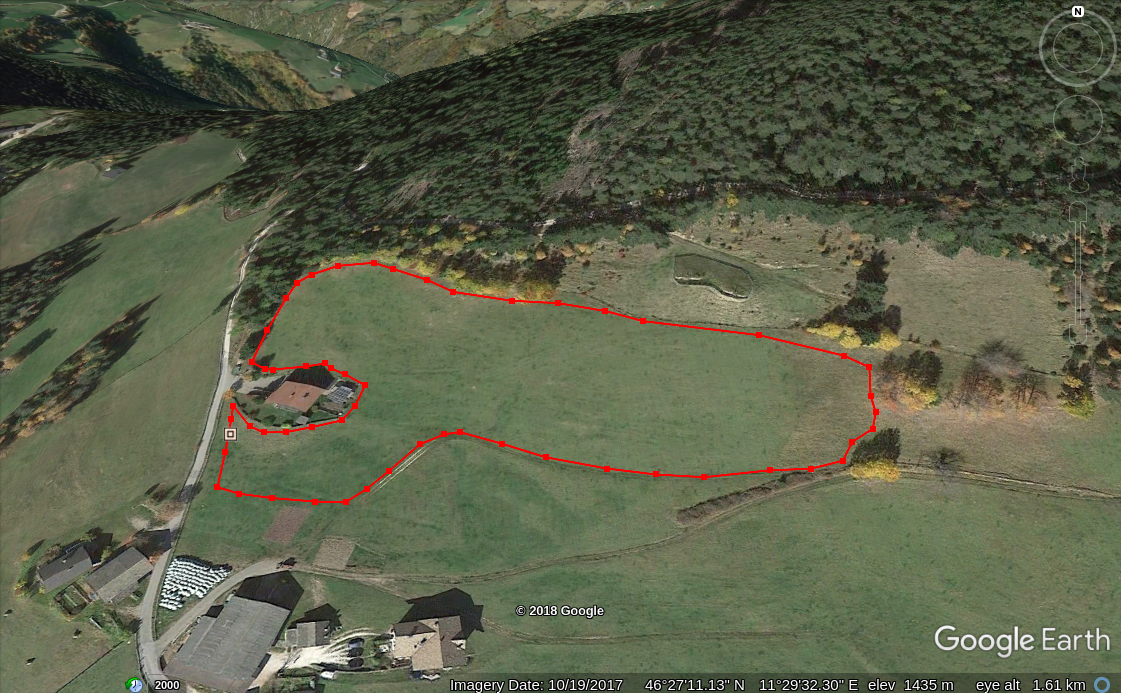
\includegraphics[width=0.9\textwidth]{figures/C2/waldpeter-boundary-GE.png}
    \caption{KML LineString geographic feature visualize on Google Earth}
    \label{fig:waldpeter-boundary-GE}
\end{figure}

\section{Implementation} % (fold)
\label{sec:implementation}
As it was accennato in \ref{sub:ortho_rectification} although the source of the orthophoto used in the software implementation is Google Earth, in defining the mission it has been taken into account the possibility to ??shut?? a photo of the whole field and georeference it (that is the goal of \textsf{/optical\_cam} node). This would provide a ??more?? up-to-dated and eventually more accurate image, but at the same time the orthophoto generation is computationally heavy especially for a mini PC. This in addition to the limited flight time of the quadcopter suggest to use Google imagery database.
In the following section it is explained how this part of the mission has been implemented in \acrshort{ros}. The most relevant part concerns the representation of the field contour as \acrshort{ros} message and the way to import it given the respective KML file.

\subsection{ROS Nodes Architecture} % (fold)
\label{sub:ros_nodes}
\autoref{fig:field-detection-rqt} shows how the three \acrshort{ros} nodes (\textsf{mission\_controller}, \textsf{optical\_cam} and \textsf{mission\_controller}, \textsf{boundary\_generator} and ), displayed as ovals, communicate together through the four topics represented inside rectangles. The node named \textsf{mavros} (for more details see appendix \ref{appendix:mavros}) on the left side of the diagram, manages everything regarding the communication with the aircraft. It basically provide a \acrshort{ros} interface to read the vehicle status variables and to change the flight controller behaviors.\par
\begin{figure}[ht]
    \centering
    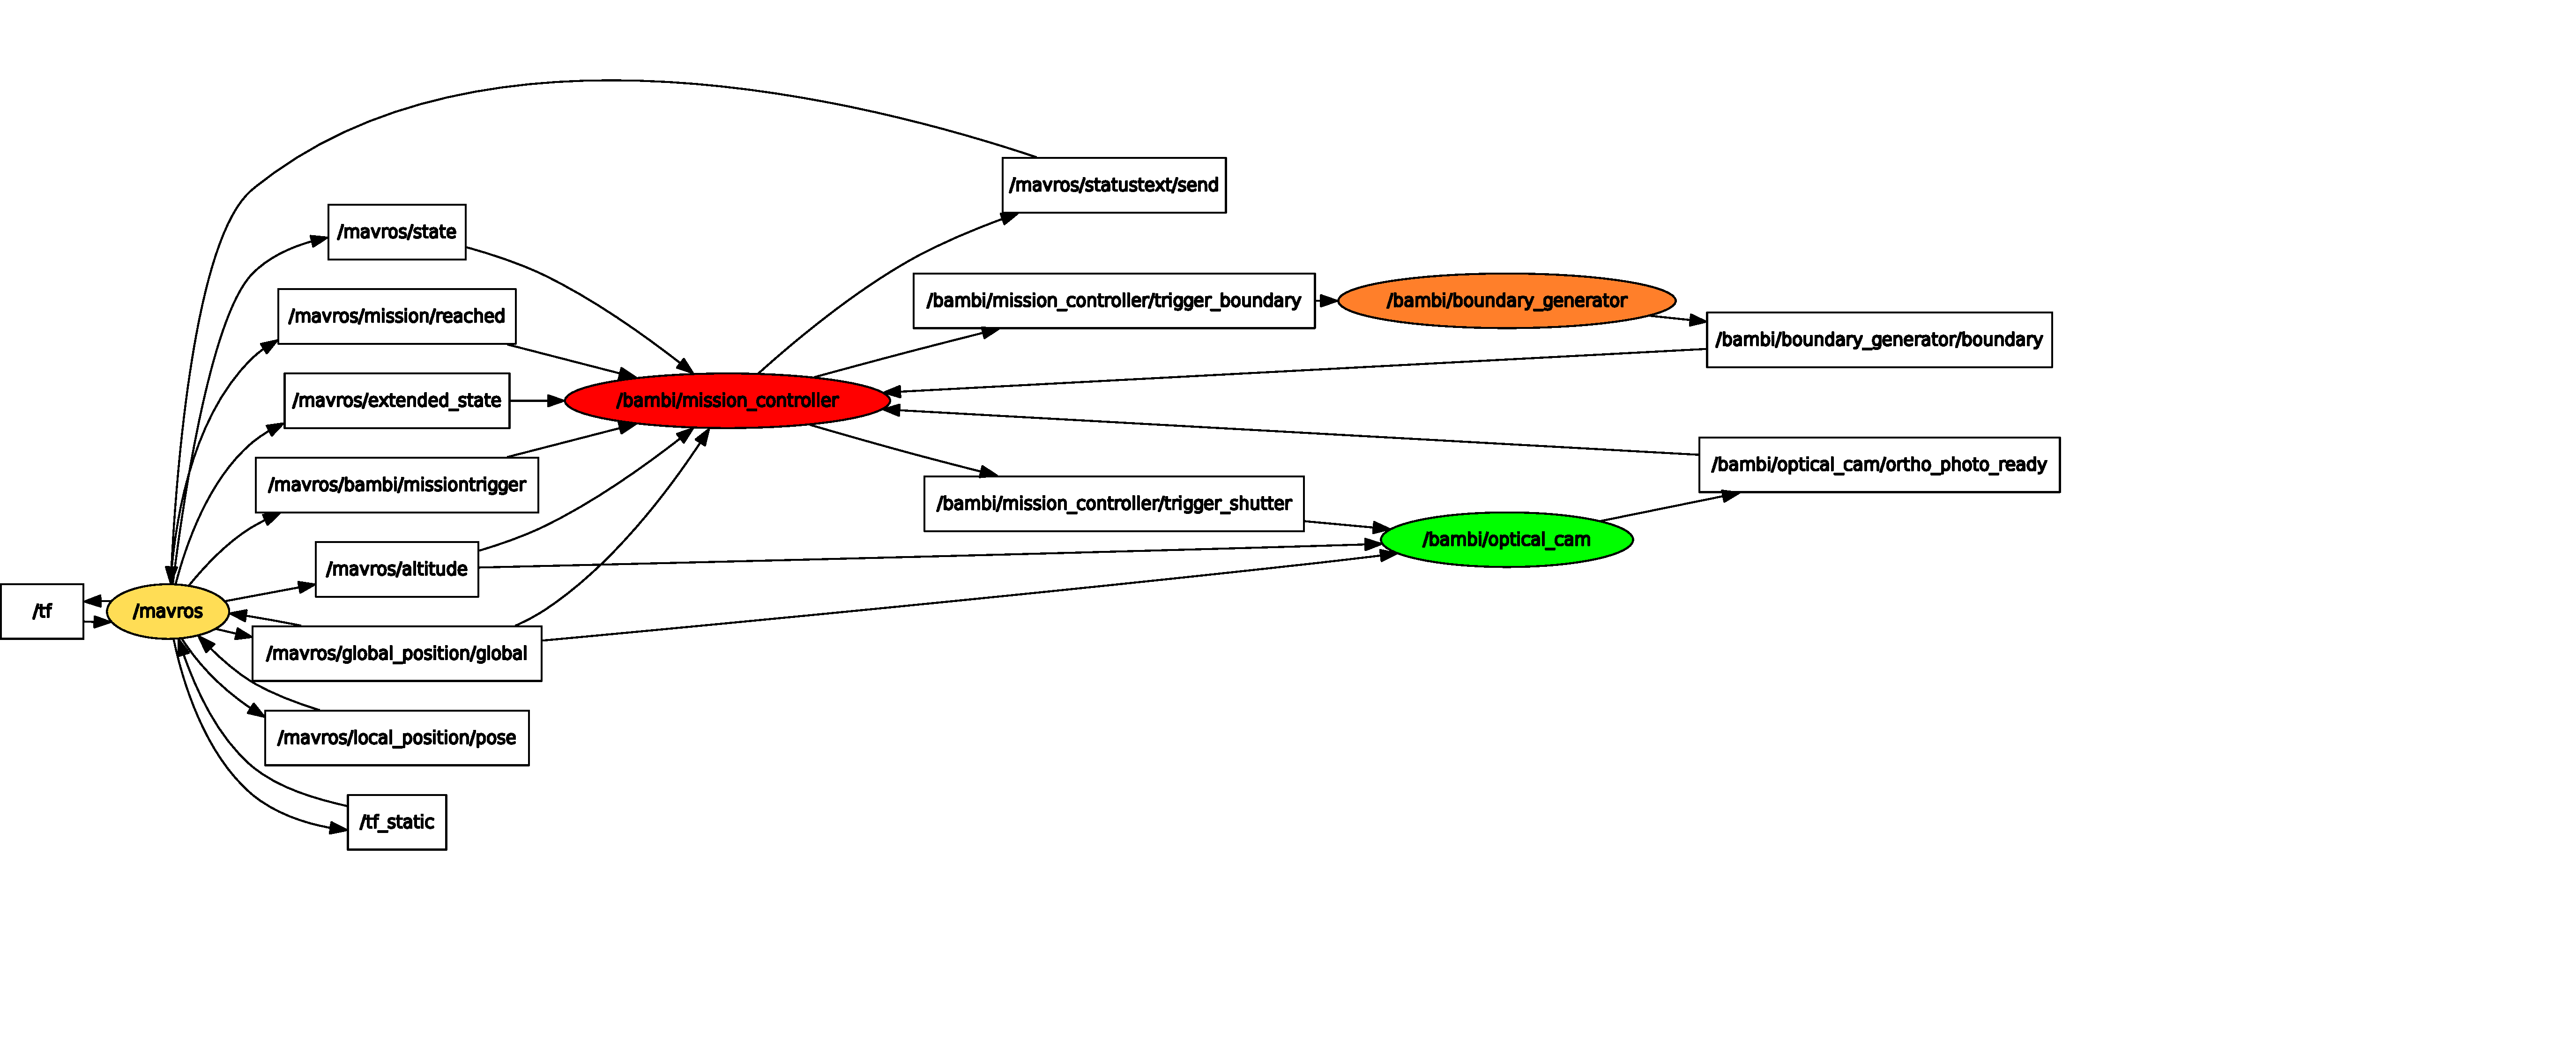
\includegraphics[width=1.3\textwidth]{figures/C2/fieldDetection-rqt_graph.pdf}
    \caption{Nodes and Topics concurring in generating the field contour}
    \label{fig:field-detection-rqt}
\end{figure}
Nodes specs:
\begin{description}
	\item[\textsf{mission\_controller}] It is the node which contains the core of the mission. Through the implementation of a finite state machine it handle every mission steps and the transition among them. For what concern the scope of this chapter the main task of this node is to trigger the other two node, which really carry out the desired tasks.
	\item[\textsf{optical\_cam}] Upon the receiving (??reception??)\todo{quale dei due termini???} of the \textsf{trigger\_shutter} message from the mission controller node it triggers the camera shutter and saves the exact GPS position required to geo-tag the photo of the field.
	At this point the node, in case the it has been chosen to georeference the image locally, will generate the orthophoto. The orthophoto algorithm has not been implemented yet as explained at the beginning of this section.
	The node finish its job once it publishes the message containing the position of the orthophoto back to the \textsf{/mission\_controller} node over the \textsf{orthophoto\_ready} topic. 
	\item[\textsf{boundary\_generator}] This node when triggered is suppose to elaborate the field boundary and sand it to the mission controller node. The communication happens through the two topics \textsf{trigger\_boundary} and \textsf{boundary} as shown in the nodes graph.
\end{description}
\subsubsection{Relevant message definitions} % (fold)
\label{ssub:relevant_message_definitions}
The definition of relevant messages is given in \autoref{list:msg-ortho}.
\lstinputlisting[label=list:msg-ortho, caption=Relevant ROS message definition, language=Python]{listings/C2/relevant-ros-messages.msg}\par

Now that a briefly introduction of each node has been done, a deeper analysis of the \textit{/optical\_cam} node and \textit{/boundary\_generator} node is carried out.
% subsubsection relevant_message_definitions (end)


\subsubsection{optical\_cam} % (fold)
\label{ssub:optical_cam}
This node has been written in python and it is responsible of the communication between the action camera (Xiaomi Yi Cam) and the other nodes running on the companion computer (raspberry Pi 3b). The camera communicate through WIFI in a server-client like fashion using the TCP protocol. For this reason, in python, the communication is managed using \textit{socket} library.
Once the socket is connected it is possible to send a several different command (in the form of \textit{token}) to remotely control the camera.\\
The first task of the node is to trigger the camera shutter when requested by the mission controller. The image is fetched and downloaded to the internal storage of the Raspberry, as soon as the camera sends back the message which tells it has successfully taken the photo. All this logic is implemented in the function \textit{take\_photo} listed in \autoref{list:camera_photo}. Most of the credits goes to Res Andy for its great effort in reverse engineering the Yi Cam remote control protocol and to provide sample scripts in python. \cite{YiCamGit}
Along with the trigger command, the node continuously listen to the topic \textit{/mavros/global\_position/global} where mavros node publishes the global position communicated by the flight controller (GPS fix). In this way the node has the necessary information to geo-tag the photo.
Once the photo is geotagged and made available locally on the onboard computer the \textit{optical\_cam} node would be in charge of generating the orthophoto. This part, at first place, has been omitted and ??leaved?? to future developments.
% \pagebreak
\lstinputlisting[label=list:camera_photo, caption=take\_photo() function in python, language=python]{listings/C2/camera_photo.py}
% subsubsection optical_cam (end)

\subsubsection{boundary\_generator} % (fold)
\label{ssub:boundary_generator}
As for \textit{/optical\_cam} node, python has been chosen as programming language because of the libraries available.
The \textit{/boundary\_generator}'s goal is, when requested, to publish \acrshort{ros} message ("Field.msg") over the topic \textit{boundary} containing the array of 2D coordinates representing the field contour.
In the following implementation the boundary information is taken from a KML file containing the geographic path manually generated through Google Earth. It has been decided to make a separated for this simple parsing task so that in future it will be ready to hold any image processing algorithm to autonomously extrapolate the field outline from the orthophoto.
The code of this node is integrally reported in \autoref{list:boundary_generator}.\\
First of all the node subscribes to \textit{/mission\_controller/trigger\_boundary} in such a way that upon the arrival of a trigger message the callback function \textit{cb\_boundary\_trigger} is called. The callback function get the absolute path of the KML file from the message attribute \textit{filenameWithFullPath}. Now it comes to play the pyKML library.\\
pyKML is a Python package for creating, parsing, manipulating, and validating KML documents \cite{pyKML}. It is based on the \textit{lxml.objectify} API \footnote{It aims to hide the usage of XML behind normal Python objects, sometimes referred to as data-binding. It allows you to use XML as if you were dealing with a normal Python object hierarchy.\cite{lxml}} which provides access to XML documents in python program. Once the file has been opened it is possible to access to KML child member in the way shown at line 23 \todo{assicurarsi si possa riferirsi cosi'}. At this point it is just a matter of parsing each geographic point as it was a string in the form "<latitude>, <longitude>" using the function \textit{split(',')}.
Latitude and longitude coordinate for each point of the contour is then packed in a geoPosition2D object which is push back on the boudary\_path vector. Once every point has been parsed and the vector filled the \textit{Field} \acrshort{ros} message is published completing the node's job.
\lstinputlisting[label=list:boundary_generator, caption=boundary generator
 node in python, language=python]{listings/C2/boundary_generator.py}.

% subsubsection boundary_generator (end)

% subsubsection ros_nodes (end)

% because there is not an explanation for explain this. I have tryed to explained the most safe way to preserve the deers but the problem is all that I am not capable to explain what is happening in to myself . i trust of myself but one part of my think about the life it is not so much easy for think that i am really capable to talk about something. so finally i think that i must stop
%  my self to try to find some origins about something when I am not capable to talk about me, this thesis is another why to try to discover  about something that it is outward rather than something that are inside me. most of people are used to talk about different things around the world because for every man it is easier to talk about something that no concern about it self. they were more years that the most part of people thinks only about everything that concerns the world outside. the fact is that it is so difficult talk about himself. this is the reason why everybody tryes to write a test that no concern about himself. il fatto è mike che studiando tutto cio mche compete il mondo tu inevitabilmente perderai parte di te stesso. come evitare cio ricorda in ogni cosa di fermarti, respirare, e sentire te stesso. annusati come faresti con un profumo nuovo. comprendi ogni cellula di te stesso per comprendere cio che ami e vuoi. e così avverra che in ogni cosa in cui ti dedicherai ilcentro non sara perdibile poiche sara sempre la parte di te che in quel momento deciderai di far uscire, esprimere e essere.

% subsection field_border_in_kml (end)




% section border_detection_and_representation (end)

 
% chapter georeferencing_the_mission_s_environment (end)


\chapter{Coverage Path Planning} % (fold)
\label{cha:coverage_path_planning}
%!TEX root = bambi-thesis.tex

\textit{Coverage path planning} (CPP) is the problem of finding a trajectory for a mobile robot such that a target area is completely swept by the sensor footprint. In the following section it is first presented the conventional CPP algorithms in use for mobile robots. Later, the focus moves more specifically over aerial application showing some previous work regarding this topic.


\section{Theory Background} % (fold)
\label{sec:theory_background}
Here a quite extensive explanation of the existing CPP algorithms will be done.

\subsection{Flight Altitude} % (fold)
\label{sub:flight_altitude}
How to compute the required flight altitude (resolution + sensor footprint + required photo overlap). Some calculation will be listed.
% subsection flight_altitude (end


% section theory_background (end)

\section{Proposal Solution} % (fold)
\label{sec:proposal_solution}

Abbiamo scelto il wavefront perche' oltre ad essere abbastanza efficente computazionalmente permette di tenere conto di diverse cost function (diverse priorita' come ad esempio l'altitudine, minor number of turns, ecc...)]
% section proposal_solution (end)


\section{Implementation in ROS} % (fold)
\label{sec:implementation_in_ros}


% section cpp_algorithms (end)
% chapter coverage_path_planning (end)

\chapter{Simulation Results} % (fold)
\label{cha:simulation_results}
%!TEX root = bambi-thesis.tex
% \section{Simulation Results} % (fold)
% \label{sec:simulation_results}
The PX4 flight stack firmware offers a great \acrfull{sitl} simulation environment which was fundamental in develop the software. In fact, it provides a real-time, safe and convenient way to test the software implementation without all the risks related to a real flight. \\

\section{Simulation Environment} % (fold)
\label{sec:simulation_environment}
The simulation environment consist of:
\begin{itemize}
 	\item \textbf{PX4 \acrshort{sitl}}: The PX4 simulated hardware which reacts to the simulated given input exactly as it would react in the reality and issues the output as a percentage of the total thrust that every rotor has to provide.
 	\item \textbf{Gazebo}: The dynamics simulator that is used by the SITL. This software reads the PX4 output and, by elaborating the modeled dynamics, provides the simulated input to the PX4. This allows for a quite accurate simulation of the real model behavior during flight.
 	\item \textbf{\acrshort{ros}}: the robotics middleware over which the Bambi Project software (in the form of package) runs.
 	\item \textbf{\acrshort{qgc}}: the ground control station used to send the mission start/stop (see appendix \ref{appendix:mavlink}) command and to monitor all the \acrshort{uav} parameters during flight.
 \end{itemize}
 The different parts of the system (\autoref{fig:SITL-architecture}) are connected via UDP, and can be run on either the same computer or another computer on the same network. The communication protocol is MAVLink (see appendix \ref{appendix:mavlink}). \\
 The following simulations has been carried out on a single PC running Ubuntu 16.04 LST.
 \begin{figure}[ht]
    \centering
    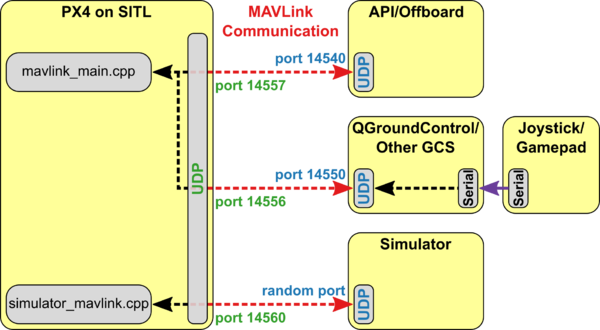
\includegraphics[width=.7\textwidth]{figures/C4/Px4_sitl_overview}
    \caption{SITL with Gazebo architectural scheme}
    \label{fig:SITL-architecture}
\end{figure}

Gazebo offers the possibility to load a satellite map through the \textsf{StaticMap} plugin\footnote{documentation at \url{http://gazebosim.org/tutorials?tut=static_map_plugin&cat=build_world}}. In this way the simulation environment (\autoref{fig:gazebo-Map}) represents quite accurately the real world scenario.
The vehicle used in simulation environment is the 3DR Iris (\autoref{fig:gazebo-iris}), because its model was already created by PX4 team along with different sensors like the 2D 360\degree\ lidar that was used to test object avoidance.
\begin{figure}[ht]
  \centering
  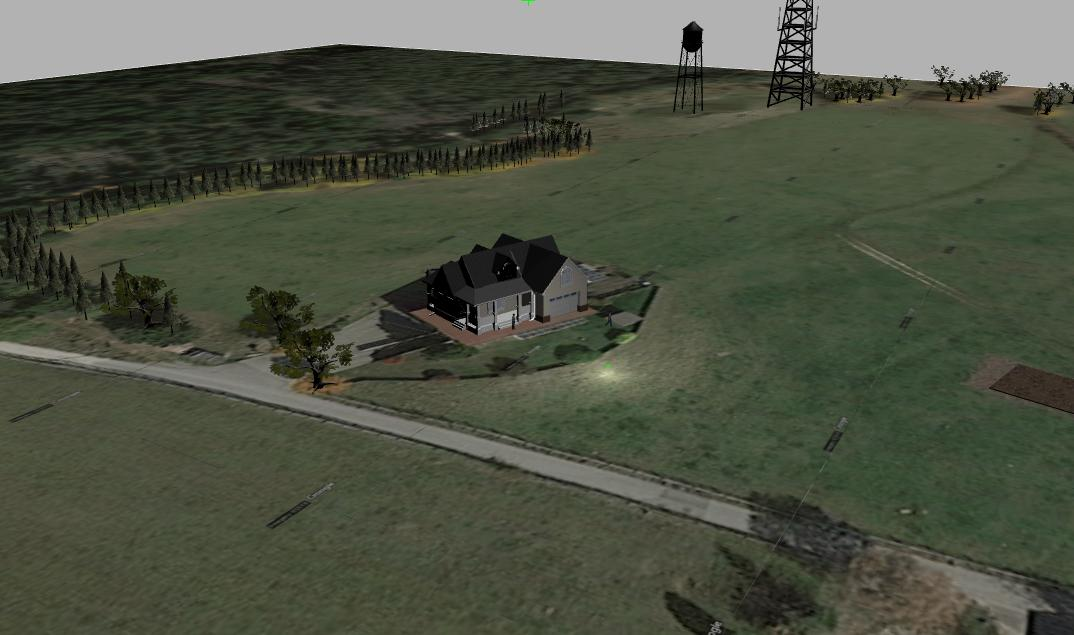
\includegraphics[width=.7\linewidth]{figures/C4/simulation/gazebo-bambi-world.jpg}
  \caption{Gazebo satellite ground plane}
  \label{fig:gazebo-Map}
\end{figure}
\begin{figure}[ht]
  \centering
  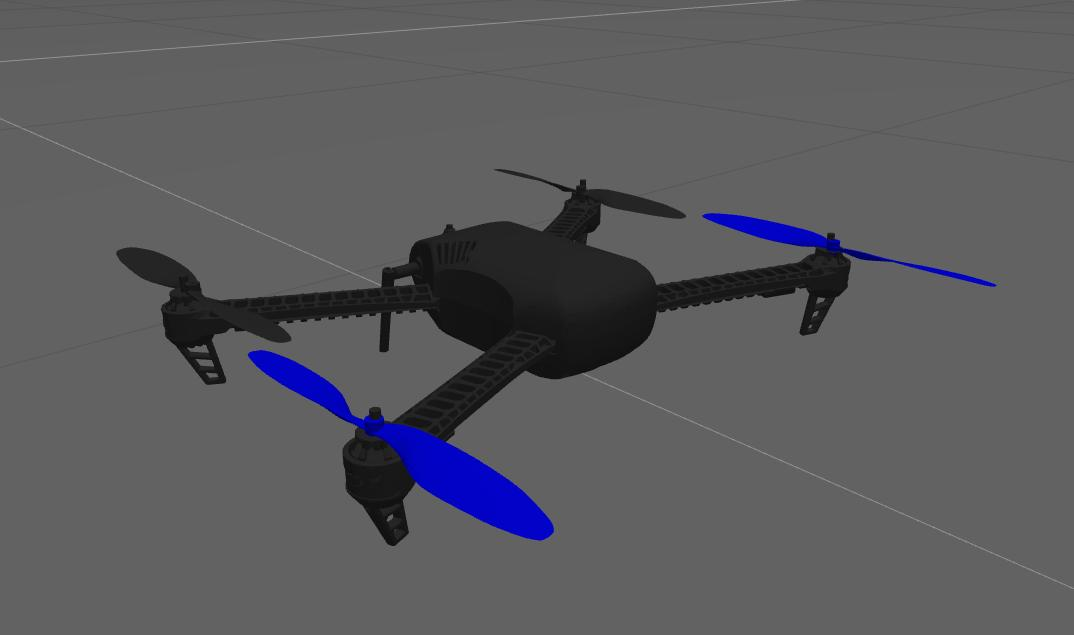
\includegraphics[width=.5\linewidth]{figures/C4/simulation/iris-model1.jpg}
  \caption{Gazebo 3DR iris model}
  \label{fig:gazebo-iris}
\end{figure}
% section simulation_Environment (end)

\section{Starting Bambi Mission} % (fold)
\label{sec:starting_bambi_mission}
Mission start and stop command are issue using the \acrshort{qgc} custom command widget displayed in \autoref{fig:qgc-widget}. This widget was written in \acrfull{qml} an user interface markup language providing an easy way to write simple GUIs \cite{QML}.\\
The button \textsf{BAMBI MISSION START} automatically send the mission start message while \textsf{BAMBI MISSION STOP} send the mission abort message which according to the current mission state causes the \acrshort{uav} to return to the home position or to immediately land at the current position.
\begin{figure}[ht]
  \centering
  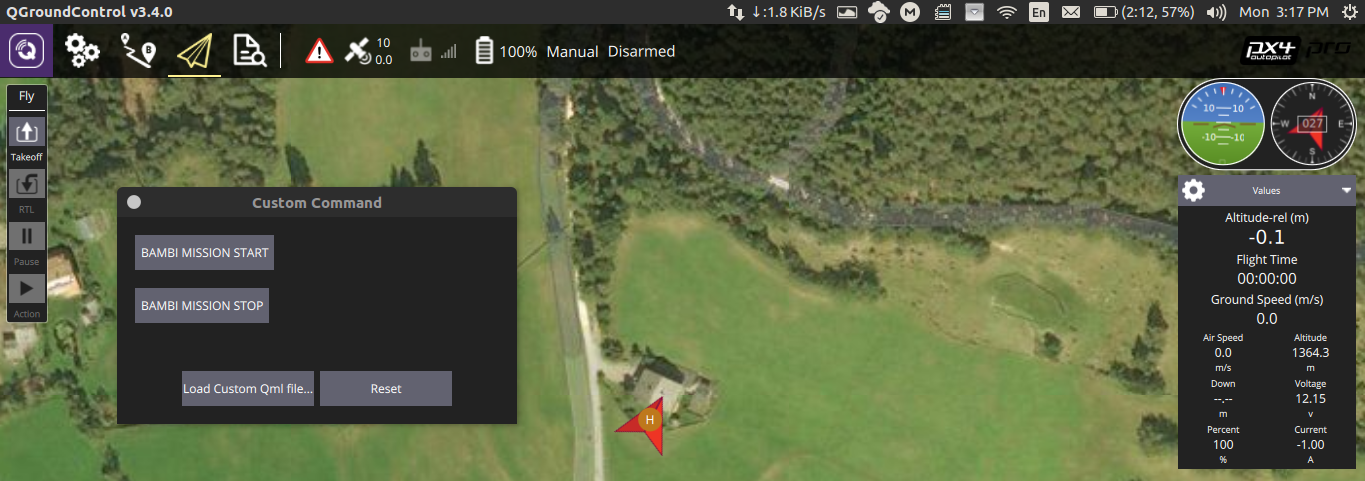
\includegraphics[width=.9\linewidth]{figures/C4/simulation/qgc-widget.png}
  \caption{QGC Bambi's custom command widget}
  \label{fig:qgc-widget}
\end{figure}
% subsection starting_bambi_mission (end)

\section{Testing CPP algorithm} % (fold)
\label{sec:testing_cpp_algorithm}
In order to test the \acrlong{cpp} algorithm it would be necessary to run through the whole mission steps and until the mission controller issue the \textsf{FieldCoverageInfo} message triggering the \acrshort{cpp} node. Therefore to save the time required by the drone to perform the first mission tasks it is convenient to publish a "fake" message directly over the \textsf{/bambi/mission\_controller/trigger\_path\_generation} topic. This is performed executing a simple bash script calling the \textsf{rostopic pub} command.\par
The algorithm was tested using different sample fields. The results obtained for three of them are displayed in \autoref{fig:Coverage-pathGE}. The cellular decomposition consist of $10 \times 10$ cells. \autoref{tbl:fields-area-length} reports the path length compared to the field area which as expected is greater for larger fields.

\begin{table}[ht]
\centering
\begin{tabular}{|l|l|l|}
\hline
\multicolumn{1}{|c|}{\textbf{Field}} & \multicolumn{1}{c|}{\textbf{Area}} & \multicolumn{1}{c|}{\textbf{Path Length}} \\ \hline
1                                    & $15444\, m^2=1.5444\, ha$          & $2.17\, Km$                               \\ \hline
2                                    & $50665\, m^2=5.0665\, ha$          & $5.56\, Km$                               \\ \hline
3                                    & $41586\, m^2=4.1586\, ha$          & $4.66\, Km$                               \\ \hline
\end{tabular}
 \caption{Comparison between field extension and coverage path length}
 \label{tbl:fields-area-length}
\end{table}
\begin{figure}[ht]
	\centering
	\begin{subfigure}{.49\textwidth}
	  \centering
	  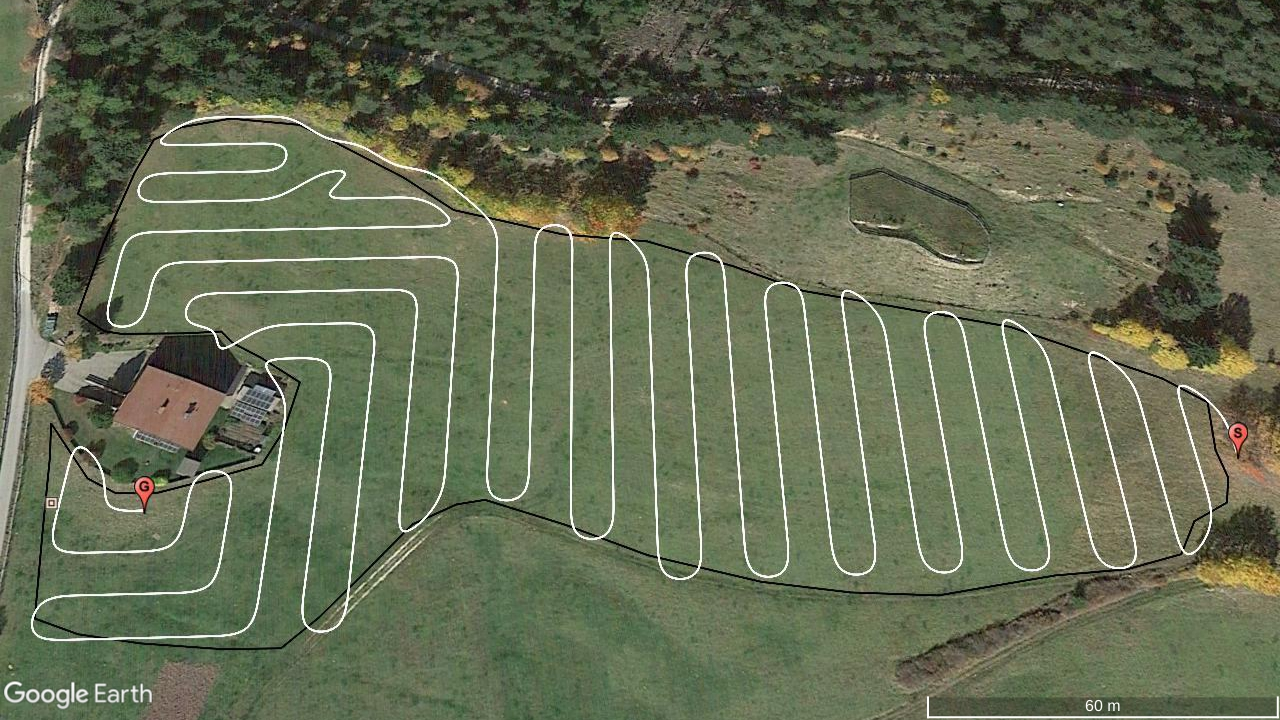
\includegraphics[width=.95\linewidth]{figures/WaldpeterField/Waldpeter-CoverageGE.jpg}
	  \caption{Field 1}
	  \label{sfig:F1-CPP-path}
	\end{subfigure}
	\begin{subfigure}{.5\textwidth}
	  \centering
	  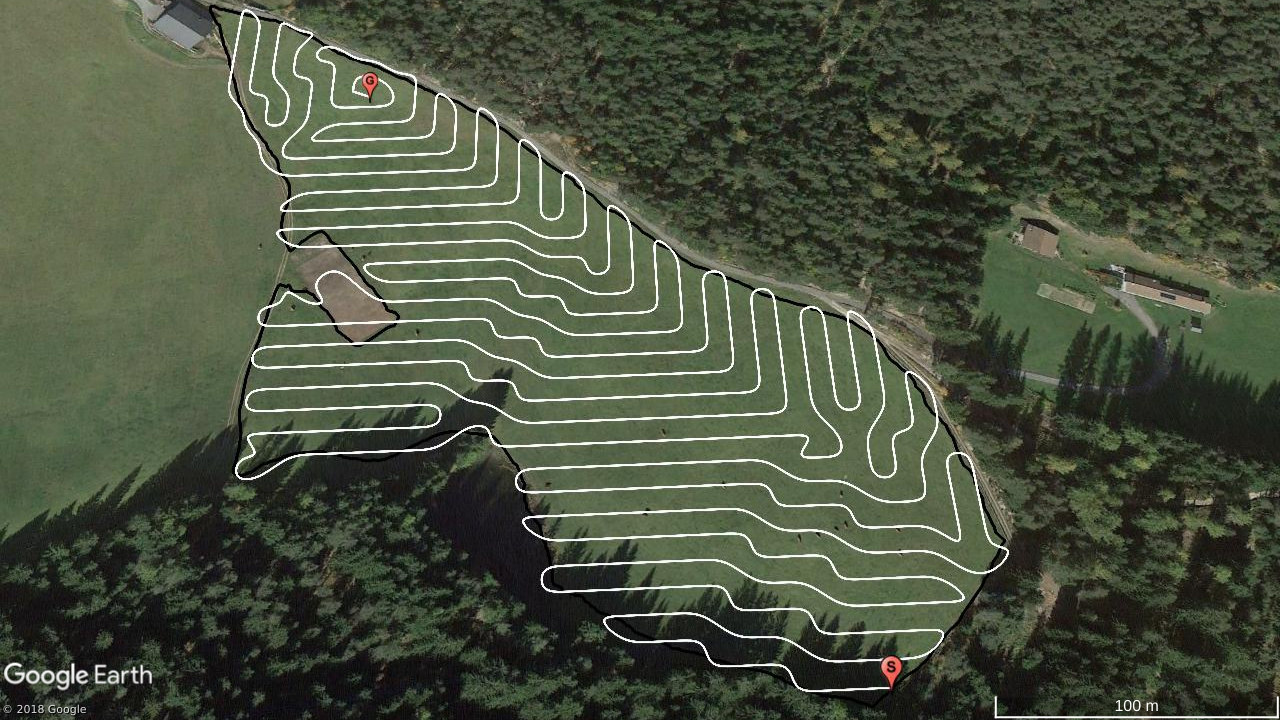
\includegraphics[width=.95\linewidth]{figures/Field2/Field2-CoverageGE.jpg}
	  \caption{Field 2}
	  \label{sfig:F2-CPP-path}
	\end{subfigure}
	\begin{subfigure}{.49\textwidth}
	  \centering
	  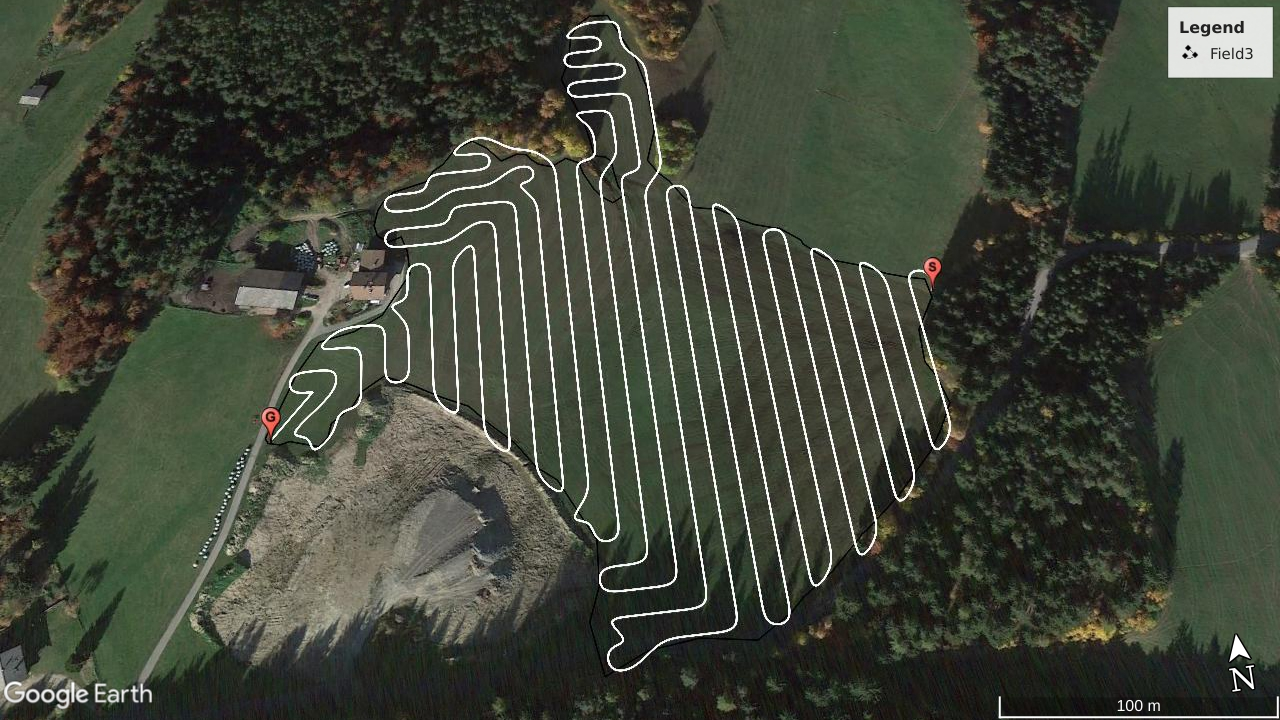
\includegraphics[width=.95\linewidth]{figures/Field3/Field3-CoverageGE.jpg}
	  \caption{Field 3}
	  \label{sfig:F3-CPP-path}
	\end{subfigure}
	\caption{CPP output path applied to different shaped fields}
    \label{fig:Coverage-pathGE}
\end{figure}
% subsection testing_cpp_algorithm (end)

\subsection{Different Starting and Goal Positions} % (fold)
\label{sub:different_starting_and_goal_positions}
During the design of {}the \acrshort{cpp} node several starting and goal position were tested. This helped to understand how the algorithm behaves under different condition and to implement a smart selection of the starting cell. \autoref{fig:coverage-start-goal-pos} shows the outcome path under three different situations.\par
When the starting point is in the middle of the field, as it is in \autoref{sfig:F3-modified-start-pos}, the coverage trajectory starts as a straight line toward the furthest point from the goal position, thought it is the path having the steepest ascending gradient. The cells visited in this transition are marked as visited and therefore avoided in the successive steps. This leads to have such kind of two halves partitioning in the trajectory.\par
The situation radically change if, at the center of the workplace, is placed the goal point. The wave-front propagate all around this position and the generated path assume the spiral like shape in \autoref{sfig:F3-modified-start-goal-pos}. As in the previous situation the path present numerous changes of direction.\par
Finally in \autoref{sfig:F3-regular-start-pos} the starting cell is chosen looking for the farthest most isolated cell with the method presented in \autoref{sub:choosing_starting_position}. The goal position is instead at the extremity of the field and it coincides with the home position, thus the point where the \acrshort{uav} were placed when the mission started. This is reasonable as, in a real situation, where the grass is tall, the mission is suppose to start from the field's border. The resulting path is definitely the best of the three showing a lawnmower like behavior. The prevalence of straight lines limits speed variations, consequently acceleration and power consumption are reduced.
\begin{figure}[ht]
	\centering
	\begin{subfigure}{0.49\textwidth}
	  \centering
	  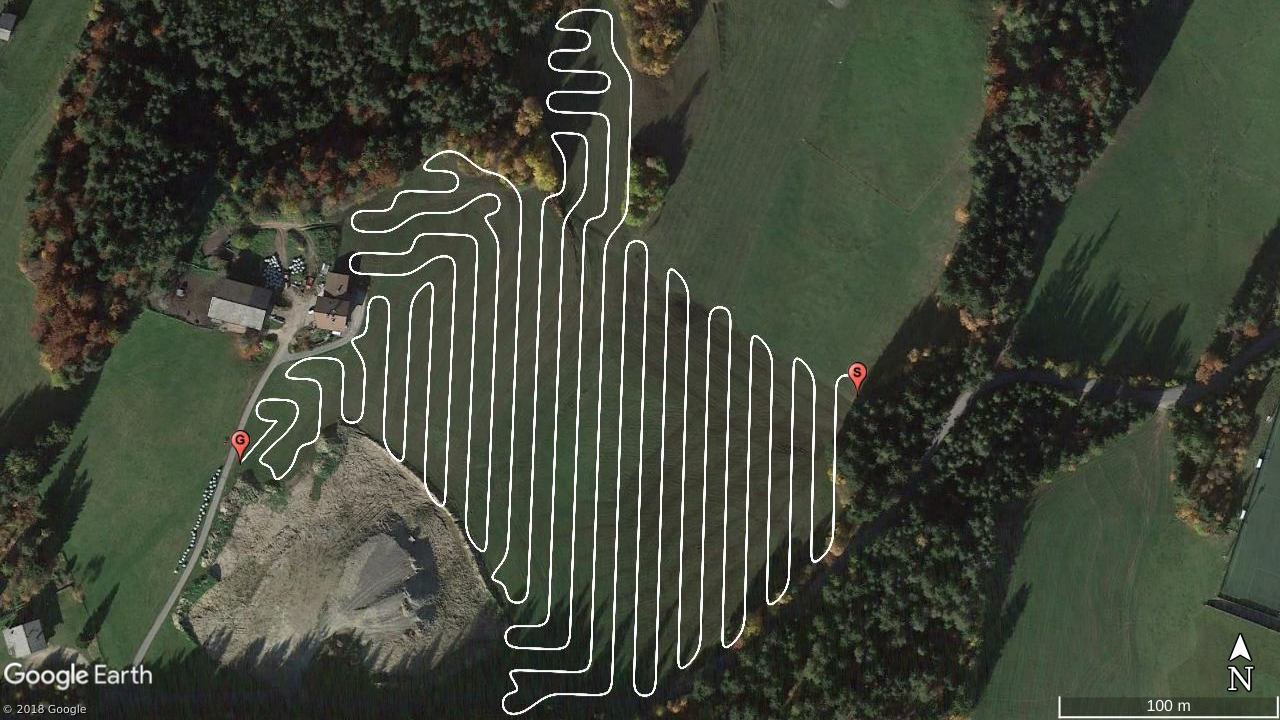
\includegraphics[width=0.95\linewidth]{figures/Field3/Field3-CoverageGE-BSpline-noBorder.jpg}
	  \caption{}
	  \label{sfig:F3-regular-start-pos}
	\end{subfigure}
	\begin{subfigure}{0.49\textwidth}
	  \centering
	  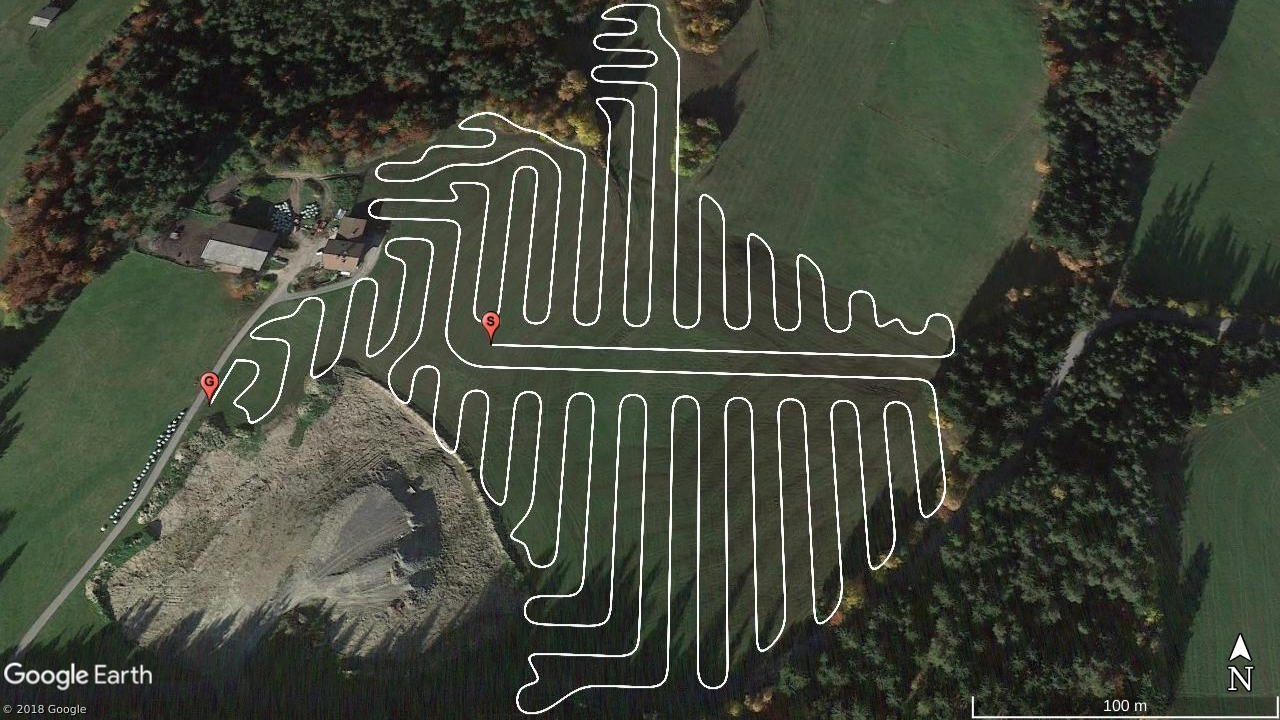
\includegraphics[width=0.95\linewidth]{figures/Field3/Field3-CoverageDifferentStartingPosition.jpg}
	  \caption{}
	  \label{sfig:F3-modified-start-pos}
	\end{subfigure}
	\begin{subfigure}{0.49\textwidth}
	  \centering
	  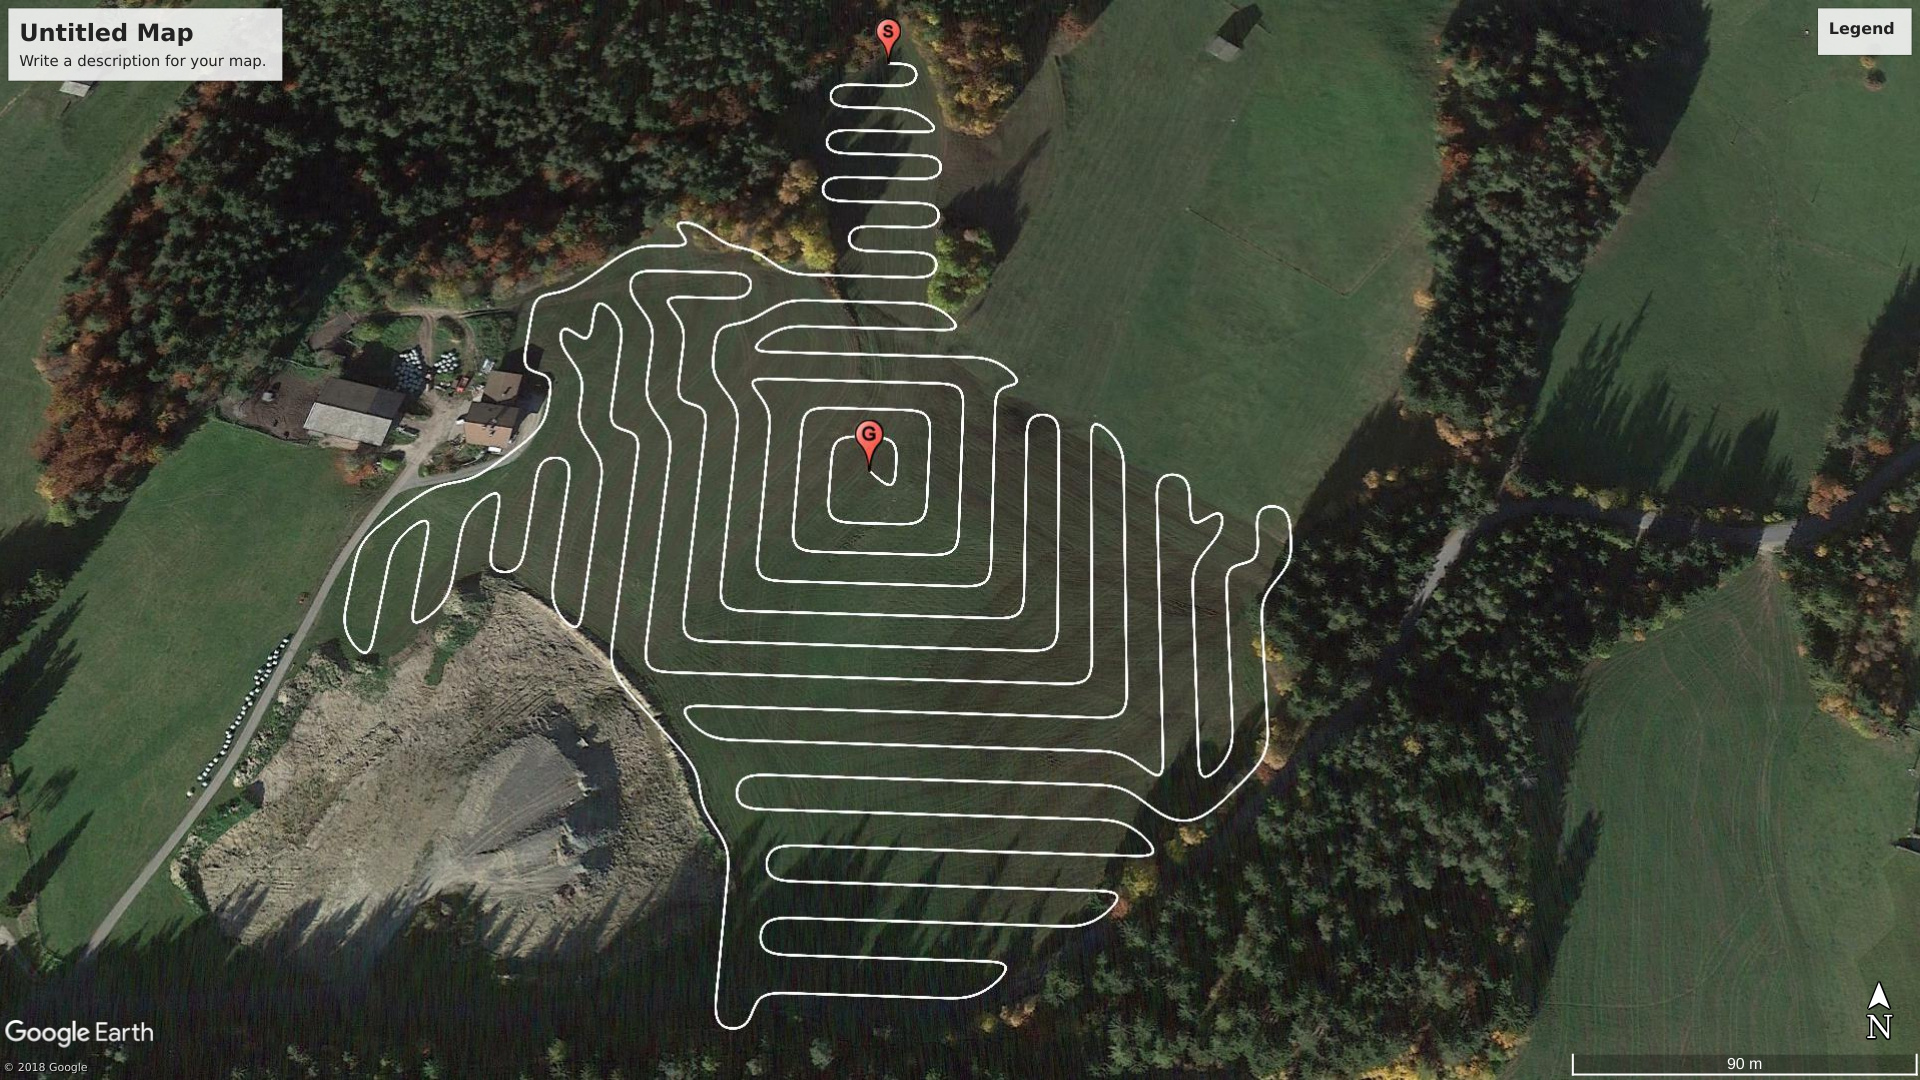
\includegraphics[width=1\linewidth]{figures/Field3/Field3-CoverageDifferentStartingGoalPosition.jpg}
	  \caption{}
	  \label{sfig:F3-modified-start-goal-pos}
	\end{subfigure}
	\caption{Coverage Path generated with Starting and Goal position}
    \label{fig:coverage-start-goal-pos}
\end{figure}
% subsubsection different_starting_and_goal_positions (end)
\subsection{Errors Analysis} % (fold)
\label{sub:errors_analysis}
Looking at the three coverage paths in \autoref{fig:Coverage-pathGE} one can notice that in some section at the border, the trajectory exceed the boundary (represented as black line). This phenomenon is a drawback of the approximate cellular decomposition (see \autoref{sub:approximate_cellular_decomposition}. The algorithm, in fact, marks a cell as part of the field when the intersection between the square polygon of the cell and the field polygon
exist. This cause the cells locate at the edge of the workplace to be marked as field even if just a small portion of them are actually inside the field. This approximation leads to imperfections in the path as shown in \autoref{fig:CPP-imperfections}. The larger are the cells, the greater becomes the effect because the approximation gets worse. For instance using $10 \times 10\, m$ cells the trajectory goes outside the border of a distance as high as $9\, m$.\par
Possible \textit{solutions} could be:
 \begin{enumerate*}
	\item Using a grid with smaller cell,thus increasing the sensor overlap;
	\item Considering a threshold on the intersecting area under which the cell it is no considered as part of the field. This could lead to a not complete coverage of the target area.
	\item In the algorithm handle external cells as particular case and using as waypoint not the center but a point inside the workplace.
\end{enumerate*}

\begin{figure}[ht]
	\centering
	\begin{subfigure}{.49\textwidth}
	  \centering
	  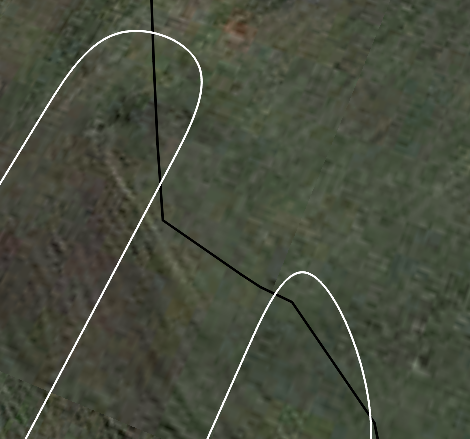
\includegraphics[width=.9\linewidth]{figures/Field3/Field3-imperfection.png}
	  \caption{}
	  \label{sfig:CPP-imperfection1}
	\end{subfigure}
	\begin{subfigure}{.49\textwidth}
	  \centering
	  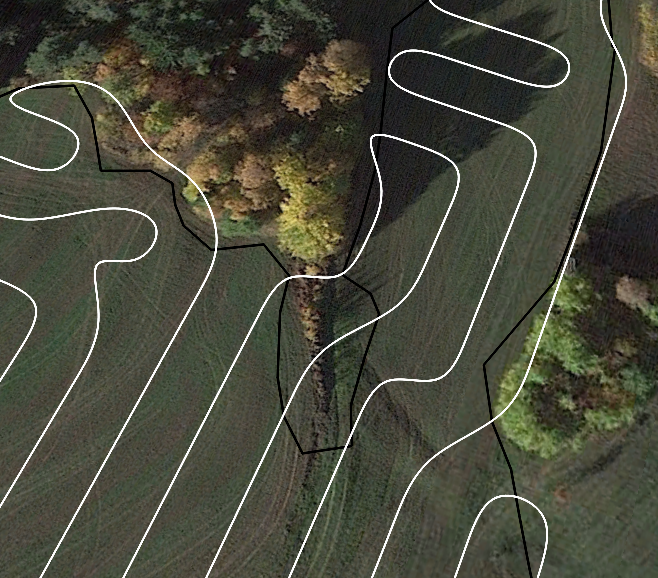
\includegraphics[width=.95\linewidth]{figures/Field3/Field3-imperfection2.png}
	  \caption{}
	  \label{sfig:CPP-imperfection2}
	\end{subfigure}
	\caption{Errors due to Approximate Cellular Decomposition}
    \label{fig:CPP-imperfections}
\end{figure}
% subsubsection errors_analysis (end)
\section{Final Considerations} % (fold)
\label{sec:considerations}
Overall, the generated path (assuming a smart selection of start and goal point) is satisfactory for the desired purpose even if, in some section, there are turns which would be nice to avoid. This is accentuated especially when the workplace has a complex shape (\autoref{sfig:F2-CPP-path}). This shortcoming is something expected, in fact, at the actual development stage, in the wave-front propagation algorithm, only the distance from the goal point is used as cost function, therefore no optimization for reducing turns has been implemented (see \autoref{sub:wave_front_propagation_algorithm}). The distance transformation used, leads to a spiral like behavior near the goal cell (discussed in \autoref{ssub:grid_based_methods}), thus it is convenient to set the goal position (home position in the mission) at an extremity of the field. \par
Regarding the issue discussed in \autoref{sub:errors_analysis}, it could cause real problem if at the border of the field there would be obstacles risking to make the \acrshort{uav} crash. This, at the actual state of development, is partially addressed relying on the \textit{object avoidance} system that has been implemented inside \textit{PX4 Firmware} which, using potential field, try to push the drone away from surrounding obstacles.\par
Finally, considering that the average flight time of a mid-range drone is between $15$ to $20$ minutes and assuming a flight mean velocity of about $4.5\, m/s$ during the mission duration, the distance it can travel is in the range of $4-5.4\, Km$. This distance is enough to cover a $4\, Ha$ field (\autoref{tbl:fields-area-length}).

% subsubsection considerations (end)


% \textit{Qui mostrero' l'output dell'algoritmo rappresentato come tracciato su google earth. verranno messi a confronto diverse scelte di starting e goal point e discutero' delle performance ottenute con relativi problemi da risolvere}

% \textit{\textbf{Mostrare importanza della scelta della starting position + bezier vs spline interpolation}}
% section simulation_results (end)


















 % Da mettere nel corpo della tesi NON INTRO

% \section{Hardware Setup} % (fold)
% \label{sec:hardware_setup}
% The quadcopter (UAV) is equipped with:
% \begin{itemize}
% 	\item Pixhawk flashed with PX4 flight stack (see appendix \ref{appendix:pixhawk_flight_controller})
% 	\item NEO-M8n (GPS){}
% 	\item 3DR telemetry radio 433Hz (serial link between the UAV and the ground station)
% 	\item LidarLite V3 (altitude distance sensor) \cite{grm:lidarlite}
% 	\item Raspberry Pi 3b (Onboard computer running ROS over Ubuntu OS)
% \end{itemize} 
%  The ground station is composed by a common laptop running QGroundControl \todo{appendix or small description and features of QGC} application. The communication with the UAV uses the MAVLink protocol \cite{Mavlink} through an USB 433Hz telemetry radio .
% % section hardware_setup (end)

% \section{Software} % (fold)
% \label{sec:software}

% \todo{ROS, PX4 why we choose them}
% \todo{ROS design graph and explanation of each node}
% \todo{go deeply in ortho photo a}
% % section software (end)
% section  (end)
% chapter simulation_results (end)

% chapter simulation_results (end)
\chapter{Conclusion and Future Work} % (fold)
\label{cha:conclusion}
%!TEX root = bambi-thesis.tex
The thesis provides \todo{Usare il passato ???} an implementation approach to \textit{georeference} and \textit{digitally encode} a geographic bounded area and to intelligently plan a \textit{coverage path} satisfying specific requirements. All this is achieved using \acrshort{ros} as software framework and therefore following at best its programming philosophy (i.e. modularity and distributive computing).\par
The main objective of the first part (\autoref{cha:georeferencing_the_mission_s_environment}), is to give basic knowledge regarding georeferentiation and to provide a way to acquire, store and manipulate the field border as geographic feature using the standard \acrfull{kml} format. Acquisition is done without particular difficulties thanks to Google Earth application and its graphical tools. At \acrshort{ros} sides it was required to write a simple Python node which, thanks to the \textsf{PyKML library}, parse the geographinc informations inside the \acrshort{kml} file and convert them to a ROS message. The implementation proves to work flawlessly without particular computational overhead even for big files. The outcome, an accurate and lightweight representation of the mission environment, is the base point of the entire mission and all other component lean on it.\par
The second part (\autoref{cha:coverage_path_planning}) is related to \acrfull{cpp}, thus generates the flight trajectory for the \acrshort{uav} in a way that, once completed, guarantees the total coverage of the target area by the on-board sensor. Several approaches from the literature were analyzed and at the end it is explain the algorithm implemented in the project. The proposal solution is based on \textit{wave-front} propagation algorithm that is largely used in navigation planning for mobile robot. For the required use case it was required to modify and rethink some parts of the original algorithm so to make it generate a \textit{coverage path}. Despite there are still space to further improvements, the results are satisfactory and the path well fits the physical properties of multirotor drones. Considering, in fact, the performance obtained in simulation environment(QUI FARE IL RIFERIMENTO AL CAP/SEC simulation results), it results that the algorithm is able to generate the trajectory for all the sample fields tested, proving to be quite robust.\\
Nevertheless, imperfections are still present, as the error caused by the approximate cellular decomposition which leads, in some situation, the trajectory to exceed the workplace boundary.
This drawback is intrinsic to the chosen area decomposition approach, but it was evaluated less important then the capability of relatively easy optimization for different path features (i.e. number of turns, terrain elevation, ecc.).\par

All the Bambi Project is available as opensource software, hosted at github under \url{https://github.com/BambiSaver}.
The project wiki is available at \url{https://wiki.bambi.florian.world} where some technical documentation and instructions on how to setup the workspace and build the code are provided.

\section{Future Works} % (fold)
\label{sec:future_work}
Many different adaptations, tests, and experiments have been left for the future due to lack of time (i.e. compile the code on the raspberry required $2$ hours). Future work concerns analysis of particular mechanisms, improvements, to try different methods and exhaustive on field testing.\par
Concerning the environment representation a great improvement could be to generate the orthophoto directly on the field. This would guarantee an up-to-dated image and eventually more accurate than Google Earth alternatives. A good starting point for this task could be to use \textsf{OpenDroneMap}, an open source toolkit for processing aerial drone imagery \cite{ODM}, which among other features provides the possibility to generate orthophoto. An important thing to evaluate is if the computing power of the Raspberry is enough to run this kind of images manipulation that is notoriously computationally expensive.\par
Another interesting feature, concerning image processing, would be to automatically detect the border of the field using a \textit{neural network}. This could be done through what is called \textit{semantic segmentation}\footnote{ Semantic segmentation describes the process of associating each pixel of an image with a class label (such as flower, person, road, sky, ocean, or car).}, thus to label every pixel of the target area as "field pixel". In this way the mission could be completely automated requiring almost no human interaction. Such kind of neural network would require a dataset of at least $1000$ images of different fields in order to be trained, therefore an huge amount of time as for each image the field must be manually recognized. After the training stage, the expected inference time on a Raspberry is around $300\, ms$ so perfectly feasible for the specific use case.\par
For the \acrfull{cpp}, the next step in the algorithm is to modify the cost function so that it takes care of the elevation profile provided by the already implemented \textsf{terrain\_data\_provider} node and to limit at maximum the number of turns. This requires to analyze and understand how to weight every features in order to build a coherent cost function. Once understand that, the only part that has to be changed in the \acrshort{cpp} algorithm is the wave-front propagation, i.e. where the matrix is filled according to the cost function (\autoref{cha:coverage_path_planning} \autoref{sub:wave_front_propagation_algorithm}).
% section future_work (end)
% chapter conclusion (end)


\bibliography{bambi-thesis}
\bibliographystyle{IEEEtran}


\begin{appendices}

%\chapter{Supplementary Information} % (fold)
%\label{cha:supplementary_information}
%!TEX root = bambi-thesis.tex
\chapter{ROS} % (fold)
\label{appendix:ros}
\textit{"The Robot Operating System (ROS) is an opensource software framework supporting the development of complex, but modular systems in a distributed computing environment. While the core components of ROS are highly generic, the primary focus of ROS and its ecosystem is set to the development and research of robots. The performance critical parts of the framework are written in C++, but applications operating on top of the framework may currently be written in C++, Python or Lisp."}\cite{7795766} \par

\section{Concepts} % (fold)
\label{sec:concepts}
\begin{description}
    \item[Master] It provides name registration and lookup to the rest of the Computation Graph. Without the Master, nodes would not be able to find each other, exchange messages, or invoke services.
    \item[Nodes] are processes that perform computation. ROS is designed to be \textit{modular} at a fine-grained scale; a robot control system usually comprises many nodes. For example, one node controls a laser range-finder, one node controls the wheel motors, one node performs localization, one node performs path planning, one Node provides a graphical view of the system, and so on. A ROS node is written with the use of a ROS client library, such as roscpp or rospy
    \item[Parameter Server] It allows data to be stored by key in a central location. It is currently part of the Master.
    \item[Messages] Nodes communicate with each other by passing messages. A message is simply a data structure, comprising typed fields. Standard primitive types (integer, floating point, boolean, etc.) are supported, as are arrays of primitive types. Messages can include arbitrarily nested structures and arrays (much like C structs).
    \item[Topics] Messages are routed via a transport system with publish / subscribe semantics. A node sends out a message by publishing it to a given topic. The topic is a name that is used to identify the content of the message. A node that is interested in a certain kind of data will subscribe to the appropriate topic. There may be multiple concurrent publishers and subscribers for a single topic, and a single node may publish and/or subscribe to multiple topics. In general, publishers and subscribers are not aware of each others’ existence. The idea is to decouple the production of information from its consumption. Logically, one can think of a topic as a strongly typed message bus. Each bus has a name, and anyone can connect to the bus to send or receive messages as long as they are the right type.
    \item[Services] The publish / subscribe model is a very flexible communication paradigm, but its many-to-many, one-way transport is not appropriate for request / reply interactions, which are often required in a distributed system. Request / reply is done via services, which are defined by a pair of message structures: one for the request and one for the reply. A providing node offers a service under a name and a client uses the service by sending the request message and awaiting the reply. ROS client libraries generally present this interaction to the programmer as if it were a remote procedure call.
    \item[Bags]A format for saving and playing back ROS message data. Bags are an important mechanism for storing data, such as sensor data, that can be difficult to collect but is necessary for developing and testing algorithms.
\end{description}
\begin{figure}[ht]
    \centering
    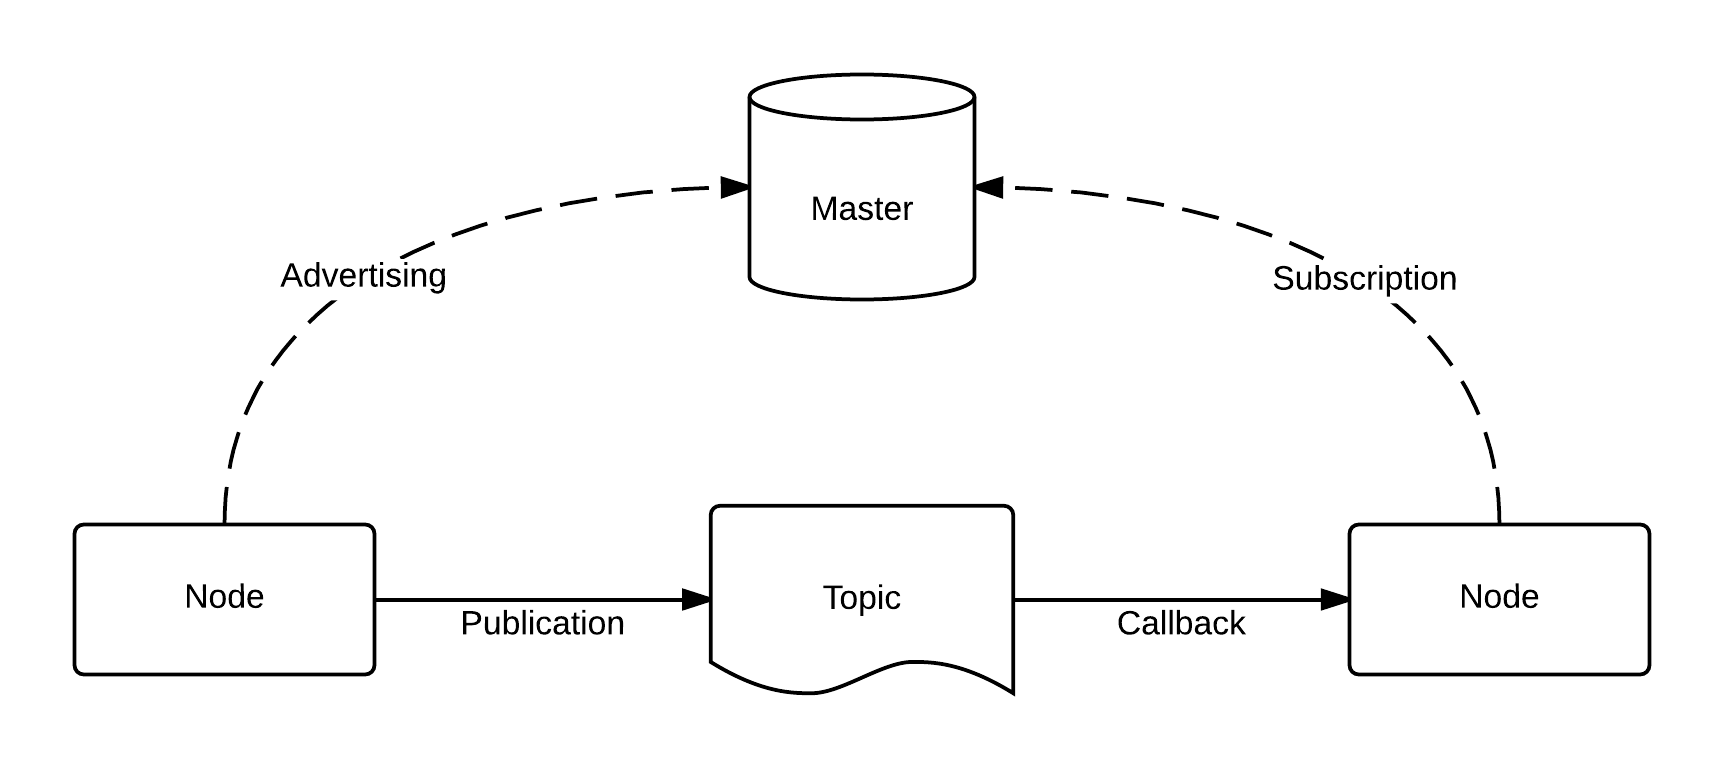
\includegraphics[width=1\textwidth]{figures/A1/ROS-master-node-topic.png}
    \caption{ROS Nodes communication}
    \label{fig:ROS-architecture}
\end{figure}
% section concepts (end)
% chapter ros (end)
%!TEX root = bambi-thesis.tex

\chapter{Pixhawk Autopilot} % (fold)
\label{appendix:pixhawk_flight_controller}
\section{Hardware} % (fold)
\label{sub:hardware}
\textit{“Pixhawk is an independent, open-hardware project aiming at providing high-end autopilot hardware to the academic, hobby and industrial communities at low costs and high availability. It provides hardware for the Linux Foundation DroneCode project. It originated from the PIXHAWK Project of the Computer Vision and Geometry Lab of ETH Zurich (Swiss Federal Institute of Technology) and Autonomous Systems Lab as well from a number of excellent individuals.”} \cite{Pixhawk}
\begin{figure}[ht]
    \centering
    \includegraphics[width=.6\textwidth]{figures/A2/pixhawk.jpg}
    \caption{}
    \label{fig:Pixhawk Flight Controller}
\end{figure}

The Pixhawk hardware weights 38g and it is provided with a 32-bit ARM Cortex M4 core with FPU with 256 KB of RAM and a 32-bit fail-safe co-processor; it is also equipped with a compass, a barometer, an accelerometer and a gyro sensor. 
% section hardware (end)

\section{Softwere} % (fold)
\label{sub:softwere}
Modern, sophisticated flight controllers share a commonality in architecture. We can divide their functionality into three distinct layers, illustrated in \autoref{fig:FCU-architecture}.
\begin{figure}[ht]
    \centering
    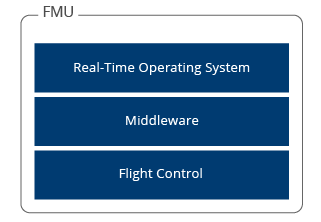
\includegraphics[width=.5\textwidth]{figures/A2/flightControllerArchitecture.png}
    \caption{The architecture of a modern flight controller}
    \label{fig:FCU-architecture}
\end{figure}
\paragraph{Layer 1: Real Time Operating System\\} % (fold)
\label{par:layer_1_real_time_operating_system}
The real time operating system is the back bone of the flight firmware, providing basic hardware abstraction and concurrency. Real time systems are critical for flight control performance and safety, as they guarantee that flight control tasks will be completed in a certain amount of time, and are essential for the safety and time-critical performance of UAVs. Luci uses a real time operating system called NuttX, which is highly expansive and configurable.
% paragraph layer_1_real_time_operating_system (end)

\paragraph{Layer 2: Middleware\\} % (fold)
\label{par:layer_2_middleware}
The middleware is a collection of tools, drivers, and libraries that relate to flight control. It contains device drivers that handle sensors and other peripherals. It also contains flight control libraries such as RC protocols, math utilities, and control filters.
% paragraph layer_2_middleware (end)

\paragraph{Layer 3: Flight Control\\} % (fold)
\label{par:layer_3_flight_control}
The flight control layer is the brains of the operation; this layer contains all of the command and control routines. Things like state estimation, flight control, system calibration, telemetry, motor control, and other flight control aspects reside in this layer.
% paragraph layer_3_flight_control (end)

\subsection{PX4 Stacks} % (fold)
\label{par:avaiable_flight_controller}

% subsection avaiable_flight_controller_ (end)
The Pixhawk platform can be flashed with two very popular flight stack: ArduPilot and PX4.
In this thesis it has been adopted the PX4 software because:
\begin{itemize}
	\item Its software-in-the-loop (SITL) simulation is much more developed and matured.
 	\item Supports a much larger number of peripherals, including more IMU sensors, lidar, range finders, status indicators, optical flow, and motion capture units. PX4 supports the most advanced sensing peripherals for drones.
 	\item Contains advanced command and control functionality, including things like terrain estimation, and indoor flight correction.
 	\item More ubiquitous and built with advanced drone applications in mind. It can be compiled for POSIX (Linux) systems, and it can also integrate with ROS to run flight applications in a hybrid system, with some running on an underlying real-time OS, and others running on Linux using ROS to communicate.
 \end{itemize} 
 The choice was mainly driven by the more developed SITL environment and framework provided by the PX4 community and for the more advanced integration with ROS rather then a matter of performance or features, where ArduPilot stack prove to be good as well.
 The diagram in \autoref{fig:PX4-architecture} provides a detailed overview of the building blocks of PX4. The top part of the diagram contains middleware blocks, while the lower section shows the components of the flight stack.
 \begin{figure}[ht]
    \centering
    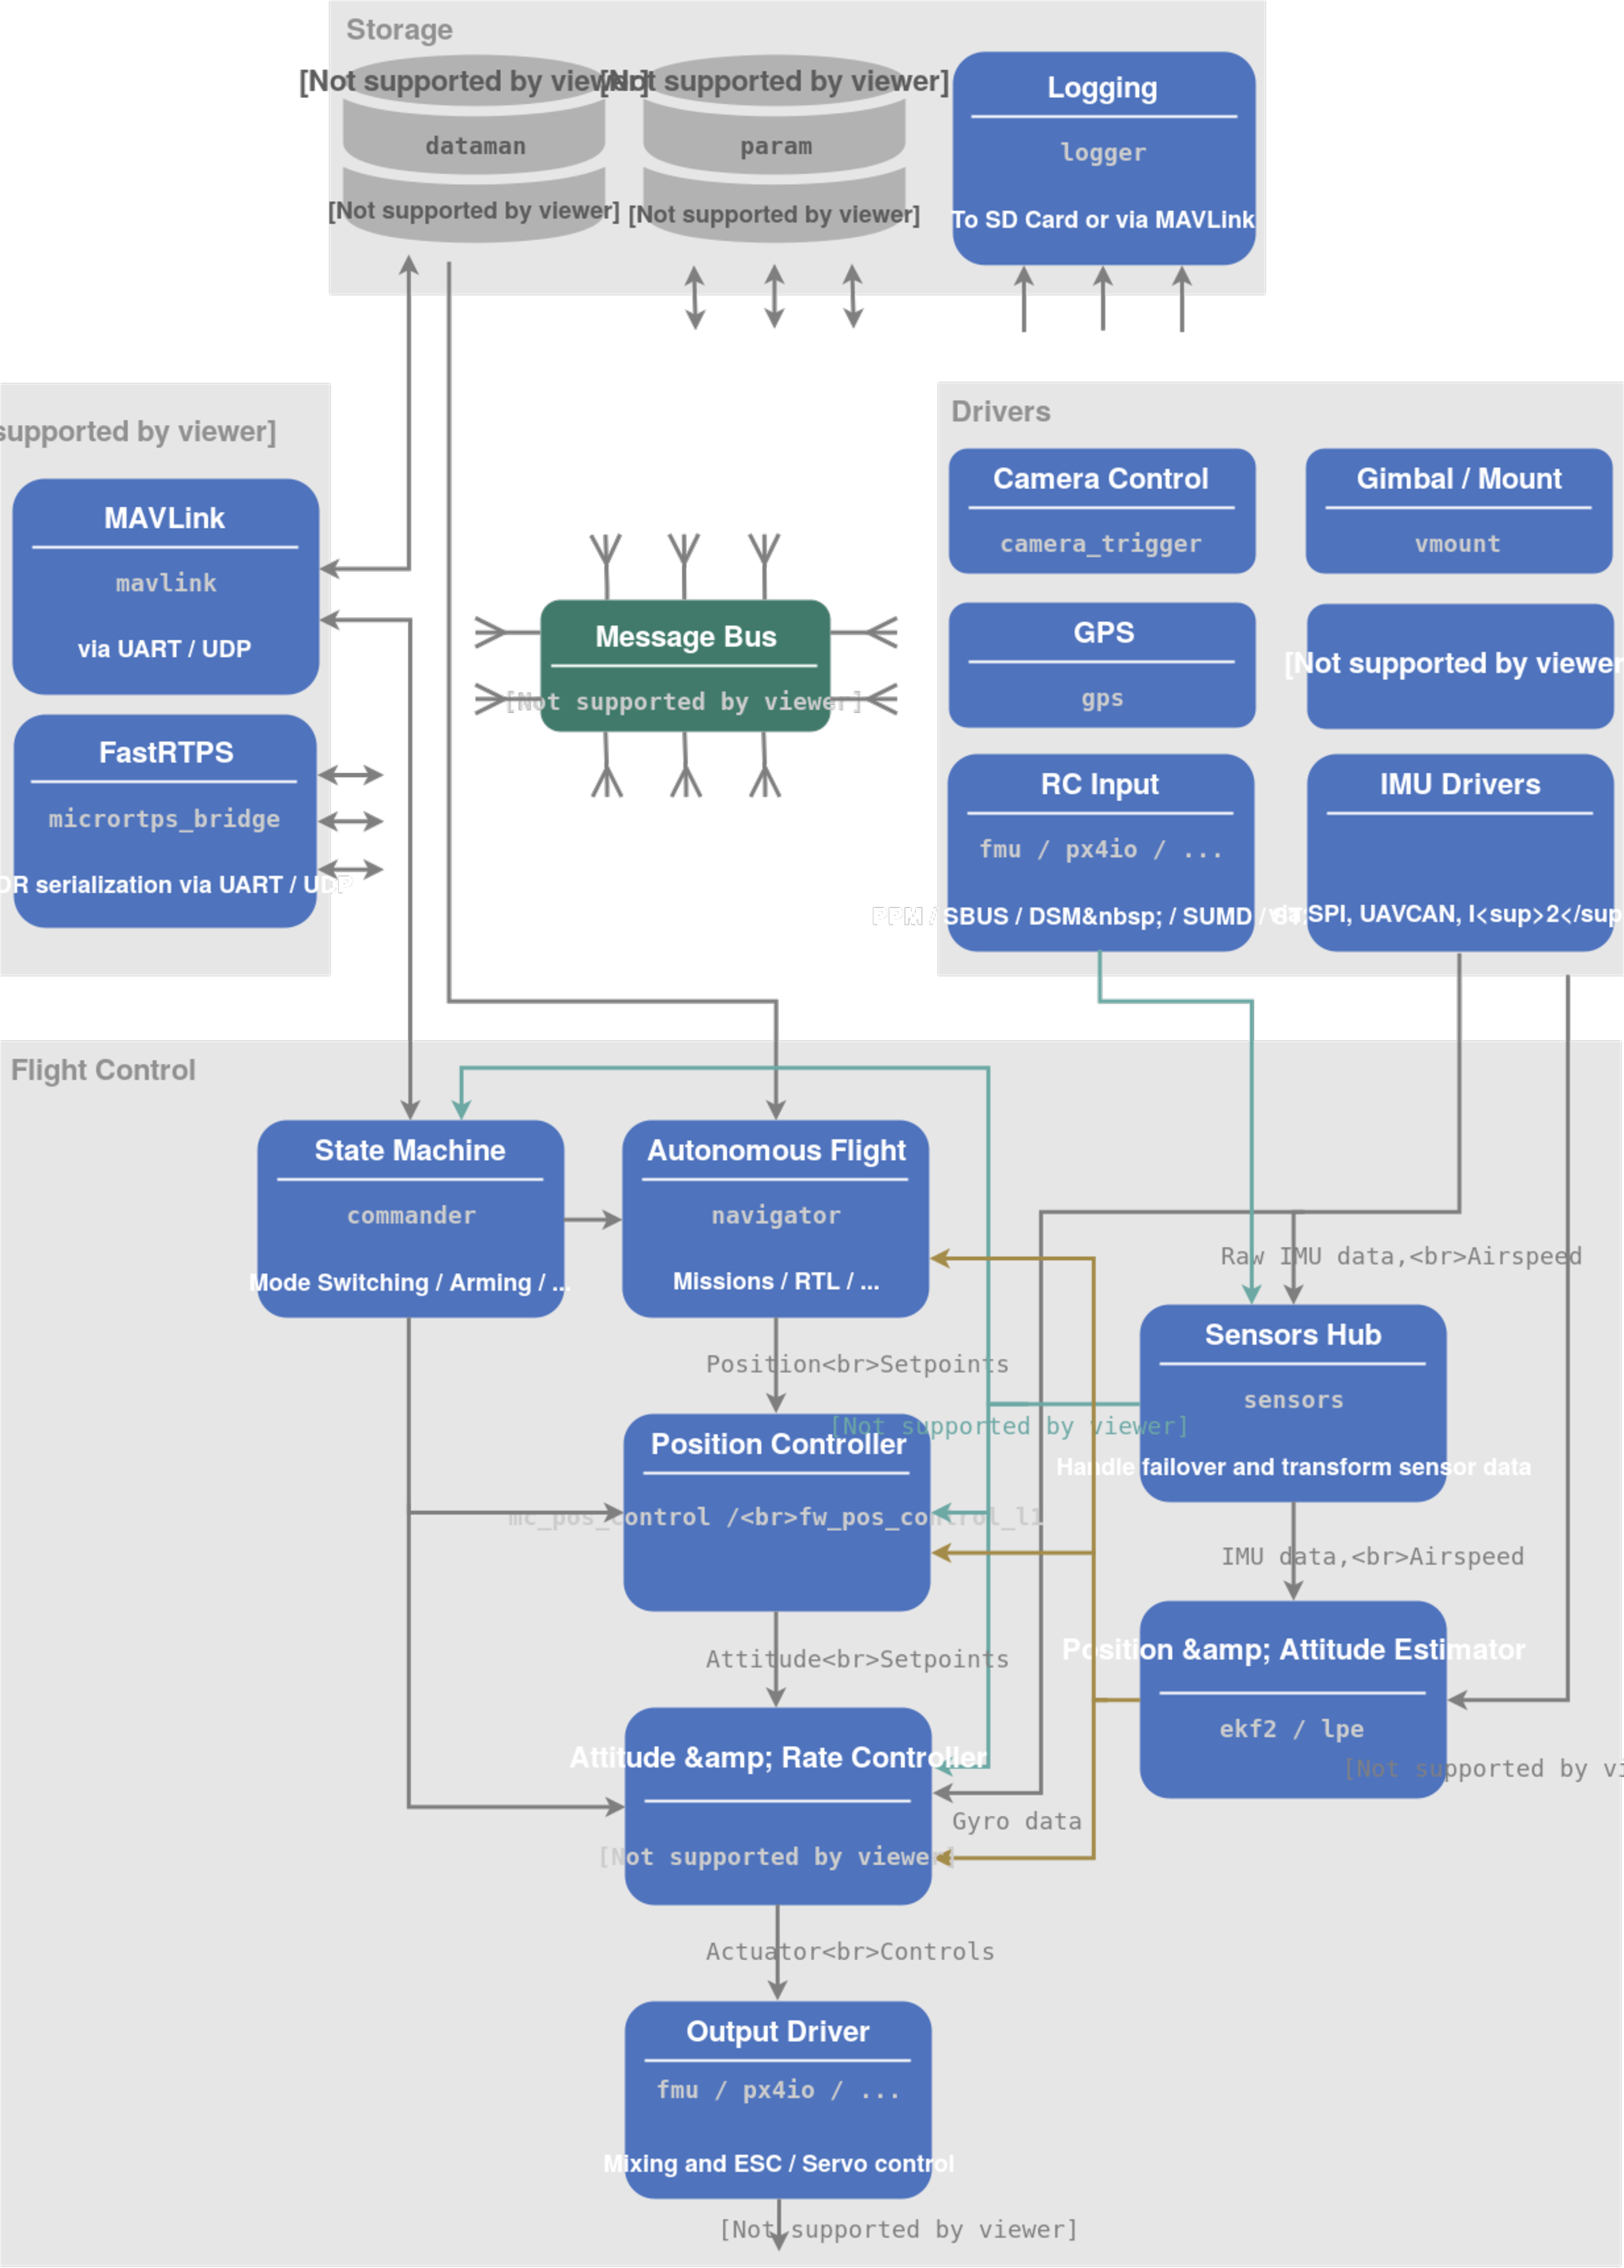
\includegraphics[width=.6\textwidth]{figures/A2/PX4_Architecture.pdf}
    \caption{PX4 Architecture}
    \label{fig:PX4-architecture}
\end{figure}
% section softwere (end)

% section pixhawk_flight_controller (end)
%!TEX root = bambi-thesis.tex

\chapter{MAVLink Protocol} % (fold)
\label{appendix:mavlink}
\textit{“MAVLink is a very lightweight messaging protocol for communicating with drones (and between onboard drone components).\\
MAVLink follows a modern hybrid publish-subscribe and point-to-point design pattern: Data streams are sent / published as topics while configuration sub-protocols such as the mission protocol or parameter protocol are point-to-point with retransmission.\\
Messages are defined within XML files. Each XML file defines the message set supported by a particular MAVLink system, also referred to as a "dialect". The reference message set that is implemented by most ground control stations and autopilots is defined in common.xml (most dialects build on top of this definition).\\
The MAVLink toolchain uses the XML message definitions to generate MAVLink libraries for each of the supported programming languages. Drones, ground control stations, and other MAVLink systems use the generated libraries to communicate. These are typically MIT-licensed, and can therefore be used without limits in any closed-source application without publishing the source code of the closed-source application.”} \cite{Mavlink}
\paragraph{Key Features} % (fold)
\label{par:key_features}
\begin{itemize}
	\item Very efficient. MAVLink 1 has just 8 bytes overhead per packet, including start sign and packet drop detection. MAVLink 2 has just 14 bytes of overhead (but is a much more secure and extensible protocol). Because \acrshort{mavlink} doesn't require any additional framing it is very well suited for applications with very limited communication bandwidth. 
	\item Very reliable. \acrshort{mavlink} has been used since 2009 to communicate between many different vehicles, ground stations (and other nodes) over varied and challenging communication channels (high latency/noise). It provides methods for detecting packet drops, corruption, and for packet authentication.
	\item Supports many programming languages, running on numerous microcontrollers/operating systems (including ARM7, ATMega, dsPic, STM32 and Windows, Linux, MacOS, Android and iOS).
	\item Allows up to 255 concurrent systems on the network (vehicles, ground stations, etc.)
	\item Enables both offboard and onboard communications (e.g. between a GCS and drone, and between drone autopilot and \acrshort{mavlink} enabled drone camera).
\end{itemize}
In  a second version of the \acrshort{mavlink} protocol was release mainly to allow more then 256 message IDs as it was in the first version. In addition MAVLink 2 is backward-compatible and implement package signing (authentication) which greatly improves security. Basic frame is shown in \autoref{fig:mavlink-packet} and each fields is described in \autoref{tbl:mavlink-frame}. There are several \acrshort{mavlink} messages. Understanding them is vital for sending proper commands to the mav.
\begin{figure}[ht]
    \centering
    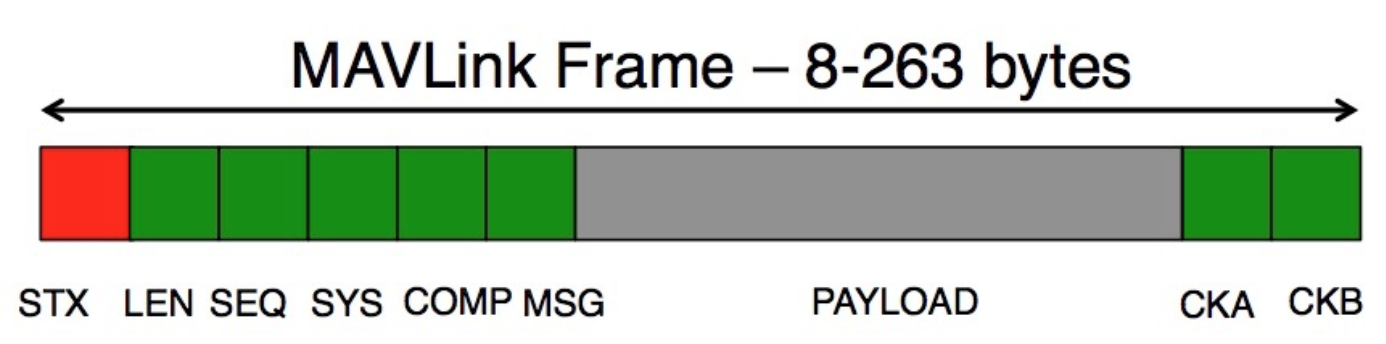
\includegraphics[width=0.6\textwidth]{figures/A3/MAVLink-frame.png}
    \caption{MAVLink packet \cite{MavlinkSerialization}}
    \label{fig:mavlink-packet}
\end{figure}

\begin{table}[ht]
\begin{tabularx}{\textwidth}{|p{1.5cm}|p{3cm}|p{1.8cm}|X|}
\hline
\textbf{Byte Index} 	&\textbf{Content}					   & \textbf{Value}     & \textbf{Description} \\ \hline 
0 						& Start byte of package                & 0xFD         		& Protocol-specific start-of-text (STX) marker used to indicate the beginning of a new packet. Any system that does not understand protocol version will skip the packet. \\  \hline
1                    	& Payload length                       & 0 - 255      		& Indicates length of the following payload section.                                                                                                                      \\  \hline
2                    	& Incompatibility Flags                &              		& Flags that must be understood for MAVLink compatibility (discards packet if it does not understand flag).                                                \\  \hline
3                    	& Compatibility Flags                  &              		& Flags ignored if not understood (implementation handle packet even if it does not understand flag). \\  \hline
4                    	& Packet sequence number               & 0 - 255      		& Used to detect packet loss. Components increment value for each message sent. \\  \hline
5                    	& System ID (sender)                   & 1 - 255      		& ID of system sending the message. Used to differentiate systems on network. \\  \hline
6                   	& Component ID (sender)                & 0 - 255      		& ID of component sending the message. Used to differentiate components in a system (e.g. autopilot and a camera).   \\  \hline
7 to 9               	& Message ID (low, middle, high bytes) & 0 - 16777215 		& ID of message type in payload. Used to decode data back into message object. \\  \hline
10 to (n+10)         	& Payload                              &              		& Message data. Depends on message type (i.e. Message ID) and contents.  \\  \hline
(n+11) to (n+12)     	& Checksum (low byte, high byte)       &              		& X.25 CRC for message (excluding magic byte). Includes CRC\_EXTRA byte. \\  \hline
(n+12) to (n+26)     	& Signature                            &              		& (Optional) Signature to ensure the link is tamper-proof. \\ \hline                                                                           
\end{tabularx}
\caption{Mavlink Packet Field Description \cite{MavlinkSerialization}}
\label{tbl:mavlink-frame}
\end{table}

\section{MAVLink Messages} % (fold)
\label{sec:mavlink_messages}
It follows a short list of the most commonly used \acrshort{mavlink} messages type:
\begin{itemize}
	\item MAVLINK\_MSG\_ID\_REQUEST\_DATA\_STREAM\\ This message is used to request the stream of data from the autopilot. Requested data can be sensors, RC channels, GPS position, status or the combination of them.
	\item MAVLINK\_MSG\_ID\_COMMAND\_LONG\\ This messa{}ge is used to give commands to the autopilot. Several commands are supported.
	\item SET\_MODE\\ It sets the different mode of operations for the drone. Few supported mode in PX4 flight stack are: \begin{enumerate*}[label=]
		\item Position;
		\item Altitude;
		\item Manual/Stabilize;
		\item Acro;
		\item Auto: Takeoff, Land, Hold, Return, Mission, Follow me, Offboard.
\end{enumerate*}
\end{itemize}
In the \textit{Bambi Project} it was necessary to define a custom \acrshort{mavlink} named \\ MAV\_CMD\_BAMBI\_ START\_STOP\_MISSION whose \acrshort{xml} definition is given in \autoref{list:mavlink-bambi}. This message is sent by the ground station (\acrshort{qgc}) to the aircraft and cause the mission state to change.
\lstinputlisting[label=list:mavlink-bambi, caption=MAVLink message definition of BAMBI\_ START\_STOP\_MISSION command, language=XML]{listings/A3/bambiMissionTriggerMAVLInk.xml}
% paragraph mavlink_messages (end)

% paragraph key_features (end)

% \begin{figure}[ht]
%     \centering
%     \includegraphics[width=.6\textwidth]{figures/A1/pixhawk.jpg}
%     \caption{}
%     \label{fig:Pixhawk Flight Controller}
% \end{figure}

%!TEX root = bambi-thesis.tex

\chapter{Mavros} % (fold)
\label{appendix:mavros}
Mavros package implements a MAVLink extendable communication node for ROS with UDP proxy for Ground Control Station that includes the following features:
\begin{itemize}
	\item Communication with autopilot via serial port
	\item UDP proxy for Ground Control Station
	\item Plugin system for ROS-MAVLink translation
	\item Parameter manipulation tool
	\item Waypoint manipulation tool'
\end{itemize}

 \begin{figure}[ht]
    \centering
    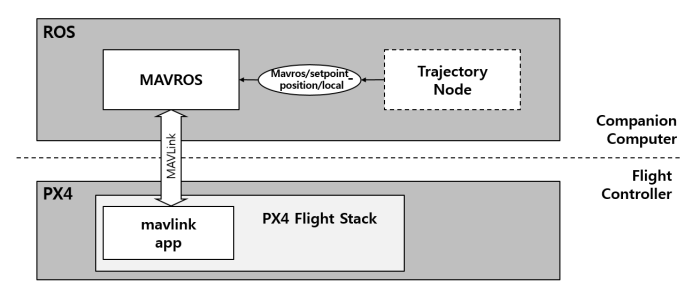
\includegraphics[width=.7\textwidth]{figures/A4/diagram.png}
    \caption{Mavros as communication gateway}
    \label{fig:mavros-diagram}
\end{figure}
Through mavros it is possible to communicate with the flight controller (\autoref{fig:mavros-diagram}) simply publishing over the topic subscribed by mavros or making a call to the services it provides.
The package is made up of various plugins, each handling different components of the FCU.
Every plugin can be load and configure separately when starting mavros through \textit{launch} file. Inside the package there are already some sample launch files specifically created to configure the communication with PX4 or APM flight stack.

% chapter mavros (end)
\end{appendices}

\pagebreak
\listoffigures
\listoftables
\listofalgorithms
\lstlistoflistings

\printindex

% chapter supplementary_information (end)




\end{document}
